\documentclass[12pt,oneside]{book}

% Маргине, проред и тако то
\usepackage[a4paper, margin=30mm]{geometry}
\renewcommand{\baselinestretch}{1.5}

% Фонтови, енкодинг
\usepackage[]{mathtext}
\usepackage[T2A, TS1]{fontenc}
\usepackage[utf8]{inputenc}
\usepackage[serbianc, russian]{babel}

\usepackage{graphicx}
\DeclareGraphicsExtensions{.pdf,.png,.jpg}

\usepackage[cmex10]{amsmath}
\usepackage{amssymb}

\usepackage[caption=false,font=footnotesize]{subfig}

\usepackage{siunitx}
\sisetup{detect-all = true,
range-phrase = --,
range-units = single,
output-decimal-marker = {,}}
\usepackage{physics}
\usepackage{nicefrac}

%\usepackage[usenames,dvipsnames,svgnames,table]{xcolor}
%\usepackage{soul}
%%\definecolor{lightblue}{rgb}{.90,.95,1}
%\colorlet{lightblue}{cyan!50}
%\sethlcolor{lightblue}

%\usepackage[nomarkers]{endfloat}%notablist,nofiglist ili nolists

\usepackage[]{foreign}

\begin{document}

\newcommand{\SkalaA}{0.1}
\newcommand{\SkalaB}{0.5}
\newcommand{\SirA}{2.0cm}
%\newcommand{\SirB}{5.8cm}
\newcommand{\SirB}{0.8\textwidth}

\newcommand{\specialcell}[2][c]{%
  \begin{tabular}[#1]{@{}c@{}c@{}}#2\end{tabular}}

\newcommand{\Fig}[1]{сл.~$\!${\ref{#1}}} 
\newcommand{\Sec}[1]{Sec.~$\!${\ref{#1}}} 
\newcommand{\blue}[1]{\textcolor{blue}{#1}}
\newcommand{\red}[1]{\textcolor{red}{#1}}
\newcommand{\comment}[1]{}


\newcolumntype{V}{>{\centering\arraybackslash} m{2cm} }

\newcolumntype{W}{>{\centering\arraybackslash} m{0.4\columnwidth} }
\newcolumntype{Z}{>{\centering\arraybackslash} m{0.44\columnwidth} }

%\chapter{Унапређено моделовање спреге сплит-ринг резонатора у штампаним колима}
\chapter{Еквивалентне шеме}

АПСТРАКТ
An enhanced equivalent circuit approach for the magnetic/electric interaction of single
split-ring resonators (SRRs) with printed lines is presented in this paper. A very simple and
efficient lumped-element network is proposed to model the behavior of metamaterial-based
printed lines over a wide frequency band. The same circuit topology can be used for the single
and two mirrored SRRs loaded microstrip line. The corresponding circuit parameters are obtained
from the multi-conductor transmission line theory as well as from closed-form expressions that
make use of just the resonance frequency and minimum of the reflection coefficient (which
should be previously extracted from experiments or full-wave simulations). The comparison of
our equivalent circuit results with measurements and full-wave simulations has shown a very
good agreement in a considerably wider frequency band than other previously proposed simple
equivalent circuits. 

\section{Увод}
Структуре за вођење таласа базиране на метаматеријалима интензивно су проучаване у протеклих деценију и по, са циљем проширења оперативних могућности различитих пасивних и активних компоненти у антенама и микроталасним колима~\cite{bib1}. Велики део труда био је посвећен проучавању штампаних водова оптерећених паралелним индуктивним и редним капацитивним елементима~\cite{bib2,bib3,bib4,caloz2005}. Резонантни водови на бази метаматеријала са двоструким СРР и комплементарним СРР резонаторима је такође разматрано у оквиру развоја филтара, сензора и RFID тагова~\cite{bib6,bib7,bib8}, између осталих примена. Једно од најзанимљивијих својстава СРР-а јесте да оријентација и положај процепа у односу на вод имају значајан утицај на особине оптерећеног вода. Ова тема је већ проучавана неким од аутора~\cite{bib9} и нашла је потенцијалне примене за пројектовање реконфигурабилних линија за кашњење и скенирајућих антена~\cite{bib10,bib11}.

Водови на бази метаматеријала (као и многе друге електромагнетне структуре) могу се адекватно моделовати помоћу еквивалентних шема са концентрисаним параметрима. Овај приступ је користан алата за боље разумевање физике ММТЛ-а. Такође, важна предност еквивалентних шема је независно подешавање параметара и оптимизација каскадираних структура. Ово и даље захтева значајно време, без обзира на огроман прогрес рачунарских перформанси, поготово ако је укључен велики број индивидуалних резонатора.

Еквивалентне шеме ММТЛ-а оптерећених са двоструким СРР-овима са карактеристикама пропусника и непропусника опсега могу се наћи, нпр. у~\cite{baena,aznar_improved}, где је копланарни таласовод (CPW) коришћен као основни вод. ММТЛ-ови базирани на микрострип воду најчешће укључују спрегу са комплементарним СРР-овима~\cite{bib14} или фракталним и вишеструким комплементарним СРР-овима~\cite{bib15} ецованим у проводној равни (испод вода), тако да се побуђују електричним пољем нормалним на раван комплементарних СРР-ова. Еквивалентна шема микрострип вода оптерећеног двоструким СРР-ом и вертикалном вијом дата је у~\cite{bib16} како би се објаснио одзив пропусника опсега. У свим претходним радовима, процепи на двоструким СРР-овима и комплементарним СРР-овима су оријентисани паралелно у односу на вод. Унакрсна спрега која резултује из другачијих оријентација била је проучавана помоћу еквивалентне шеме у~\cite{naqui:13}.

Треба приметити да се у свим горепоменутим примерима (са изузетком~\cite{bib16}) ради о двостраним структурама, које је тешко фабриковати и уклопити са другим планарним компонентама. Ова чињеница може ограничити њихову примену у савременим бежичним системима, где су редукована величина, цена и лакоћа интеграције примарни захтеви. Због ових разлога, микрострип технологија је можда најбољи избор за интеграцију ММТЛ-ова и сродних компоненти.

У овом поглављу ће се проучавати квадратни СРР-ови спрегнути са микрострип водом, који се налазе у истој равни. Процепи у СРР-овима су или паралелни (ближе или даље воду) или нормални у односу на вод, при чему ови последњи испољавају ефекат унакрсне поларизације. Разматрени су случајеви једног СРР-а са једне стране вода, или два СРР-а постављених симетрично / асиметрично на обе стране вода. Еквивалентна шема је предложена и валидирана за произвољну оријентацију једног СРР-а. Топологија кола је нешто комплекснија од досад преложених, како би се повећао фреквенцијски опсег модела. Нови модел користи исти број независних параметара као и претходни, иако су елементи повезани на другачији начин, како би се ефикасније представила дистрибуирана природа оригиналног вода. Апроксимација може бити још побољшана додавањем више елемената у репрезентацију са концентрисаним параметрима, али ово би повећало сложеност модела и број параметара које треба одредити.

Предложене јединичне ћелије испољавају одзив непропусника опсега, и могу се користити као основна компонента у пројектовању компактних филтара високих перформанси. Валидност еквивалентне шеме потврђена је помоћу $Ѕ$-параметара добијених мерењем лабораторијских прототипова и 3Д електромагнетним симулацијама. Предложена топологија кола је врло подесна и за јединичне ћелије-пропуснике опсега, зато што се индуктивност вије може лако додати без повећања сложености модела.

Организација овог поглавља је следећа: секција 2. представља екстракцију параметара кола коришћењем модела спрегнутих водова, како би се добили параметри основног вода спрегнутог са СРР-овима. У секцији 3. се одређују преостали параметри помоћу аналитичких израза који користе резонантну фреквенцију и минимум коефицијента рефлексије, добијене из симулација. Два типа еквивалентних шема су размотрена: са једном и две П-ћелије. Показано је да други случај даје око два пута већи опсег важења. Еквивалентне шеме су валидиране поређењем са симулацијама и мерењима у секцији 4. Веома добро слагање добијено је у целом опсегу, не само за структуре са једном јединичном ћелијом, него и за структуре са њиховом каскадом.

\begin{figure}[!t]
\centering
%\includegraphics[scale=0.2]{fig1}
\caption{Изглед микрострип вода спрегнутог са СРР-ом са релевантним димензијама: $h =
1.27\, \mathrm{mm}$, $L_r = 3\, \mathrm{mm}$, $L_m = 0.25\, \mathrm{mm}$, $L_g = 0.5\,
\mathrm{mm}$, $W_r = 0.2\, \mathrm{mm}$, $W_l = 1.2\, \mathrm{mm}$, $S = 0.1\, \mathrm{mm}$.
Дебљина метализације је $t =17\, \mathrm{\mu m}$, а диелектрична пермитивност $\varepsilon_r=10.2$.} 
\label{f1}
\end{figure}

\section{Екстракција параметара кола коришћењем модела спрегнутих водова}

Како би се добили модели еквивалентних кола за микрострип вод оптерећен произвољно оријентисаним СРР-овима, који могу имати процепе нормално и паралелно (ближе и даље) у односу на вод, две конфигурације су испитиване: 1) један СРР са једне стране вода и 2) два СРР-а са обе стране вода. Еквивалентна шема арбитрарно оријентисаних СРР-ова није разматрана раније, са изузетком моделовања међусобне спреге између самих СРР-ова~\cite{bib18}.

\begin{figure}[!t]
\centering
\subfloat[]{\includegraphics[scale=0.22]{sl_ekv/fig2a}
\label{f2a}\label{f3e}}\hspace{0.3cm}
\subfloat[]{\includegraphics[scale=0.26]{sl_ekv/fig2b}
\label{f2b}\label{f3f}}
\caption{Еквивалентна шема микрострип вода оптерећеног са СРР-ом, која има: (a) једну, и (b) две $\Pi$-ћелије.} 
\label{f2}
\end{figure}
Микрострип вод оптерећен СРР-ом са паралелним процепом ближе воду приказан је на \Fig{f1}, заједно са релевантним димензијама. Слична структура, али са двоструким СРР-овима, проучавана је у~\cite{bib16}, где је предложена еквивалентна шема приказана на \Fig{f2a}. Вод је представљен помоћу једне $\Pi$-ћелије. Овде се предлаже унапређени модел приказан на \Fig{f2b}, где је вод представљен помоћу две $\Pi$-ћелије. Биће демонстрирано да ово коло, које има исти број независних параметара као и претходно, омогућава много боље слагање са симулацијама и мерењима.

Како би се екстраховали параметри $L$ и $C$ вода (\Fig{f2}), узимајући у обзир спрегу између вода и најближе ивице СРР-а, систем је моделован као секција вишепроводничког вода. Програм LINPAR~\cite{djordjevic1999linpar} је коришћен за нумеричко израчунавање квази-статичких параметара вода. Као излазни подаци добијају се матрице подужних индуктивности и капацитивности, из којих се могу добити параметри секција коначне дужине.

У складу са геометријом спреге између СРР-а и вода, проучаване структуре су подељене у пет група, приказаних у табели~\ref{tab1}. У функцији од оријентације СРР-а, микрострип вод је спрегнут са целом ивицом, или два њена дела раздвојена процепом.

\begin{table}[!t]
  \centering
 \caption{Конфигурације СРР-ова спрегнутих са микрострип водом и екстраховани параметри. Спрега је узета у обзир само у шрафираним секцијама. Референтне равни су обележене тачкастим линијама.} 
  \label{tab1}
\begin{tabular}{| m{0.5cm}  | V V | m{3cm} |}
	\hline
    (а) & 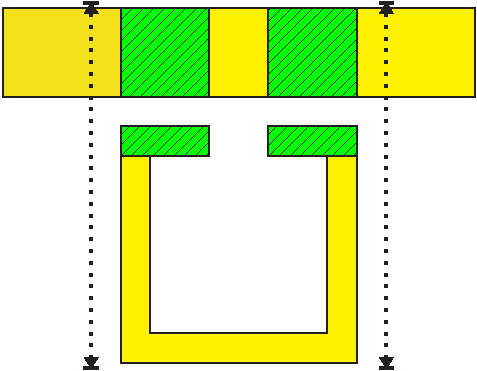
\includegraphics[width=\SirA,trim=0 0 0 -5]{sl_ekv/pod0} &  
& \parbox[t]{3cm}{$L=1.51\,\mathrm{nH}$\\$C=0.72\,\mathrm{pF}$\\$L_s=7.97\,\mathrm{nH}$}  \\ \hline
    (б) & 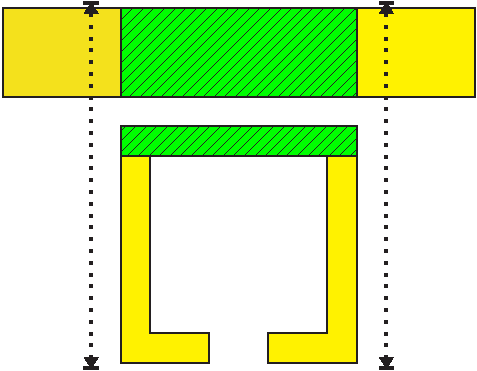
\includegraphics[width=\SirA,trim=0 0 0 -5]{sl_ekv/pod180}& 
    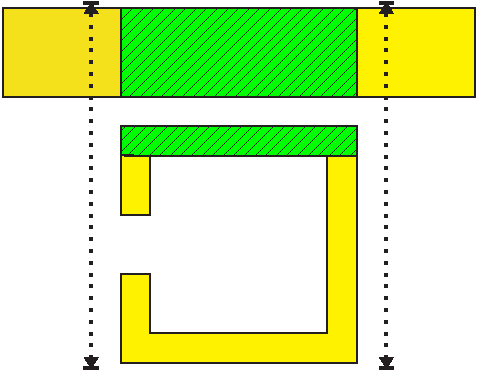
\includegraphics[width=\SirA,trim=0 0 0 -5]{sl_ekv/pod90} 
& \parbox[t]{3cm}{$L=1.51\,\mathrm{nH}$\\$C=0.74\,\mathrm{pF}$\\$L_s=7.92\,\mathrm{nH}$} \\ \hline
    (в) & 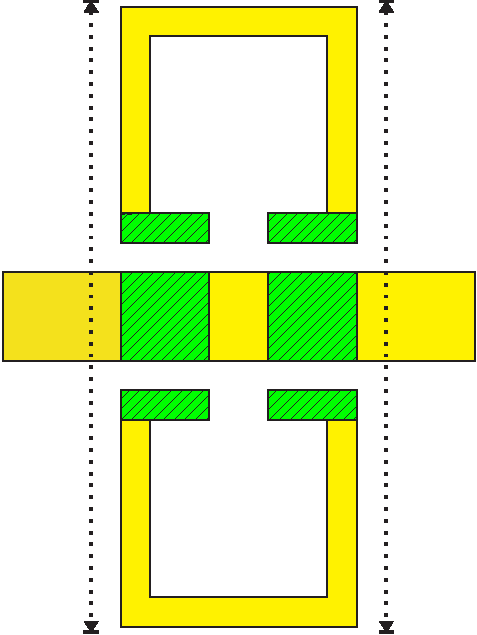
\includegraphics[width=\SirA,trim=0 0 0 -5]{sl_ekv/pod0x2} &
& \parbox[t]{3cm}{$L=1.5\,\mathrm{nH}$\\$C=0.82\,\mathrm{pF}$\\$L_s=7.97\,\mathrm{nH}$} \\ \hline
    (г) & 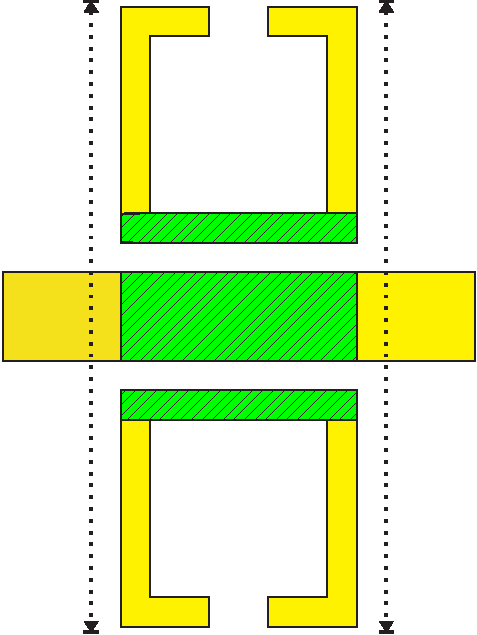
\includegraphics[width=\SirA,trim=0 0 0 -5]{sl_ekv/pod180x2}& 
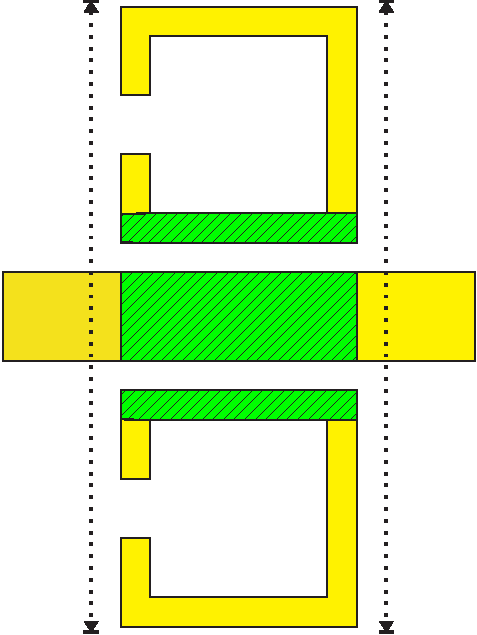
\includegraphics[width=\SirA,trim=0 0 0 -5]{sl_ekv/pod90x2} 
& \parbox[t]{3cm}{$L=1.5\,\mathrm{nH}$\\$C=0.86\,\mathrm{pF}$\\$L_s=7.92\,\mathrm{nH}$} \\ \hline
(д) & 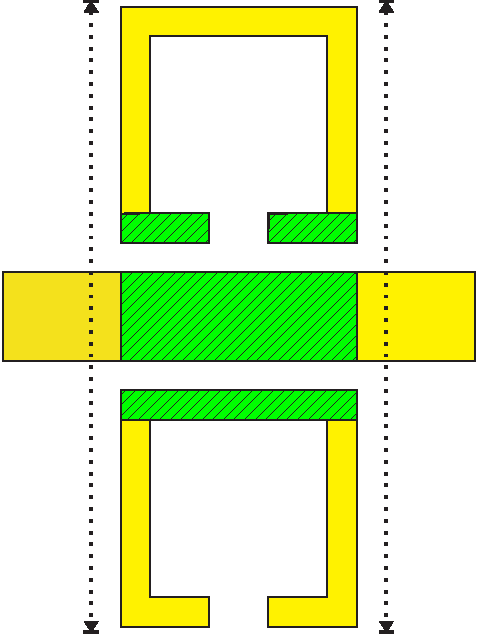
\includegraphics[width=\SirA,trim=0 0 0 -5]{sl_ekv/pod180+pod0} & 
&
\parbox[t]{3cm}{$L=1.5\,\mathrm{nH}$\\$C=0.84\,\mathrm{pF}$\\$L_{s1}=7.97\,\mathrm{nH}$\\$L_{s2}
=7.92\,\mathrm{nH}$} \\ \hline
  \end{tabular}
%\vspace{1em}
\end{table}
У табели~\ref{tab1} могу се разликовати три врсте означених секција: изоловане, и спрегнуте са једном или две ивице СРР-а. Параметри сваке секције су прорачунати коришћењем подужних вредности. Резултирајући параметри вода (дати у трећој колони табеле) добијени су сабирањем параметара индивидуалних секција. Може се видети да је индуктивност вода, $L$, врло слична у свим конфигурацијама, док капацитивност, $C$, више варира (око 15\%) у зависности од спреге. Индуктивности прстенова, $L_S$, састоје се од два дела: 1) од секције која је спрегнута са водом, која се прорачунава на основу одговарајућег елемента матрице, и 2) од изолованог вода, чија је дужина једнака преосталом, неспрегнутом делу СРР-а. Бредности $L_S$ дате у табели се нешто разликују због чињенице да спрегнута секција има нешто нижу вредност индуктивности. У наставку су усвојене исте вредности индуктивности, $L=1.5\, \mathrm{nH}$ и $L_S = 8\, \mathrm{nH}$, за све разматране конфигурације.

\section{Екстракција параметара кола на основу симулираних резултата}

Откривено је да се различите конфигурације микрострип вода спрегнутог са СРР-овима могу моделовати истом топологијом кола, само са различитим вредностима параметара. На основу топологије, све разматране конфигурације могу се поделити у три категорије:
\begin{itemize}
\item СРР са процепом паралелним воду или два СРР-а са паралелним процепима, симетричним у односу на вод,
\item два СРР-а са паралелним процепима, при чему је један процеп ближе а други даље од вода,
\item један или два СРР-а са нормалним процепима.
\end{itemize}
За сваку топологију, могу се извести аналитички изрази за резонантну фреквенцију и фреквенцију минимума рефлексије. Ови изрази ће бити искоришћени за одређивање преосталих параметара (коефицијент магнетне спреге, $k_m$, капацитивност СРР-а, $C_s$), полазећи од фреквенција добијених у нумеричким симулацијама. Једини параметар који је неопходно фитовати је коефицијент електричне спреге, $k_e$; односно међусобна капацитивност, $C_m=k_e \sqrt{CC_s }$, у случају СРР-ова са нормалним процепима (овај коефицијент је уведен у секц.~\ref{sec:ML2SPerp}). 

\subsection{СРР са процепом паралелним воду}\label{sec3:2}
Микрострип водови оптерећени са СРР-овима са паралелним процепом приказани су на \Fig{f3}.
Параметри еквивалентне шеме $L$, $C$ и $L_S$ дати су у табели~\ref{tab1} за све конфигурације са \Fig{f3} (они зависе од геометрије и карактеристика материјала). Преостали параметри, $C_S$ и $k_m$, ће бити одређени на основу $Ѕ$-параметара добијених симулацијом. Треба приметити да, у разматраном фреквенцијском опсегу, симулирани $Ѕ_{11}$ параметар поседује само један минимум испод резонантне учестаности, док еквивалентне шеме поседују два минимума: један испод и један изнад резонансе. Присуство овог паразитног минимума смањује опсег у коме је могуће добити добро слагање између симулације и еквивалентне шеме. Ипак, шема са две П-ћелије [\Fig{f2b}] помера овај минимум на више учестаности у односу на модел са једном ћелијом, о чему ће се дискутовати касније.
%\begin{figure}[!t]
%\subfloat[]{\includegraphics[width=2cm]{fig3a}
%\label{f3a}}
%\subfloat[]{\includegraphics[width=2cm]{fig3b}
%\label{f3b}}
%\addtocounter{subfloat}{2}
%\subfloat[]{\includegraphics[scale=0.18]{fig3e}
%\label{f3e}}
%\addtocounter{subfloat}{-3}
%\subfloat[]{\includegraphics[width=2cm]{fig3c}
%\label{f3c}}
%\subfloat[]{\includegraphics[width=2cm]{fig3d}
%\label{f3d}}
%\addtocounter{subfloat}{1}
%\subfloat[]{\includegraphics[scale=0.18]{fig3f}
%\label{f3f}}
%\caption{Microstrip line loaded with SRRs with gaps parallel to the line: (a) one SRR with gap
%near the line, (b) two SRRs with gaps near the line, (c) one SRR with gap far from the line,
%(d) two SRRs with gaps far from the line. These configurations can be modeled by the
%equivalent circuits (e) and (f).}
%\label{f3}
%\end{figure}
\begin{figure}[!t]
\centering
\begin{tabular}{W W}
    \subfloat[]{\includegraphics[width=0.8\linewidth]{sl_ekv/fig3a}
    \label{f3a}} &
    \subfloat[]{\includegraphics[width=0.8\linewidth]{sl_ekv/fig3b}
    \label{f3b}} \\
    %\addtocounter{subfloat}{2}
    %\subfloat[]{\includegraphics[width0.8=0.75\linewidth]{fig2a}
    %\label{f3e}} \\
    %\addtocounter{subfloat}{-3}
    \subfloat[]{\includegraphics[width=0.8\linewidth]{sl_ekv/fig3c}
    \label{f3c}} &
    \subfloat[]{\includegraphics[width=0.8\linewidth]{sl_ekv/fig3d}
    \label{f3d}} 
    %\addtocounter{subfloat}{1}
    %\subfloat[]{\includegraphics[width=\linewidth]{fig2b}
    %\label{f3f}}
\end{tabular}
\caption{Микрострип вод спрегнут са СРР-овима са паралелним процепима: (а) један СРР са процепом ближе воду, (б) два СРР-а са процепима даље од вода.} 
\label{f3}
\end{figure}

Капацитивност $C_S$ се добија из резонантне учестаности СРР-а $f_r=\omega_r/2\pi$ на следећи начин:
\begin{equation}
f_r = \frac{1}{2\pi \sqrt{L_SC_S}}\;.
\end{equation}

%%%%%%%%%%%%%%%%%%%%%%%%%%%%%%%%%%%%%%%%%%%%%%%%%%%%%%%%%%%%%%%%%%%%%%%%%%%%%%%%%%%%%
\subsubsection{Минимум $S_{11}$ испод резонансе}
%%%%%%%%%%%%%%%%%%%%%%%%%%%%%%%%%%%%%%%%%%%%%%%%%%%%%%%%%%%%%%%%%%%%%%%%%%%%%%%%%%%%%

Коефицијент магнетне спреге, $k_m$, се одређује на основу првог минимума $S_{11}$, $f_\text{min}=\omega_\text{min}/2\pi$,  за коло са \Fig{f2}. Како би се поједноставило израчунавање, биће примењена Бартлетова бисекциона теорема~\cite{bib20}. Коефицијент $k_m$ се онда добија као функција $f_\text{min}$, резонантне фреквенције$f_r$ и параметара вода $L$ и $C$,
\begin{equation}
k_m^2 = \left( 1 - \frac{\omega_r^2}{\omega_\text{min}^2} \right) \left( 1 - a_{1,2} \right) 
\end{equation}
где $a_1$ одговара колу са једном ћелијом [\Fig{f2a}], а $a_2$ колу са две ћелије [\Fig{f2b}]. Ови коефицијенти су дати са
\begin{align}
a_1 & = \left[ \frac{L}{C}Y_0^2 + 2b \right]^{-1} \\
a_2 & = \left[ \frac{L}{C}Y_0^2 \left( 1 - \frac{b}{2-b} \right) + b \right]^{-1} 
\end{align}
где је $Y_0$ карактеристична адмитанса вода ($20\,\mathrm{mS}$ у овом случају), и 
\begin{equation*}
b  = \left( \frac{\omega_\text{min}}{\omega_0} \right)^2;\quad
\omega_0^2=\frac{8}{LC}\;.
\end{equation*}
%%%%%%%%%%%%%%%%%%%%%%%%%%%%%%%%%%%%%%%%%%%%%%%%%%%%%%%%%%%%%%%%%%%%%%%%%%%%%%%%%%
\begin{figure}[!t]\centering
\subfloat[]{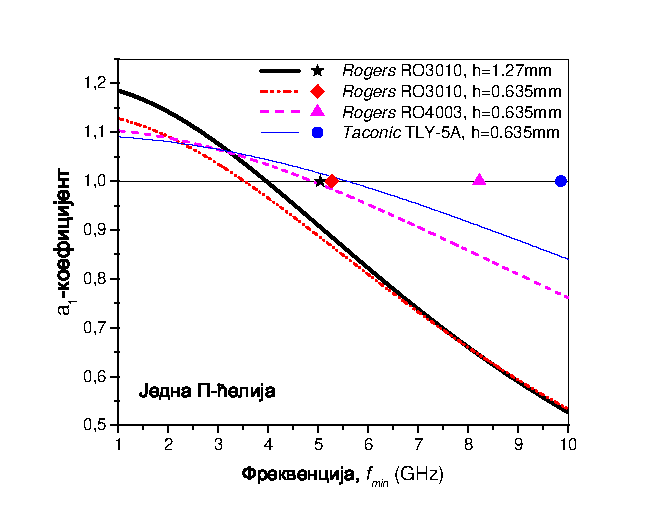
\includegraphics[width=0.8\textwidth]{sl_ekv/fig4a}
\label{f4a}}\\
\subfloat[]{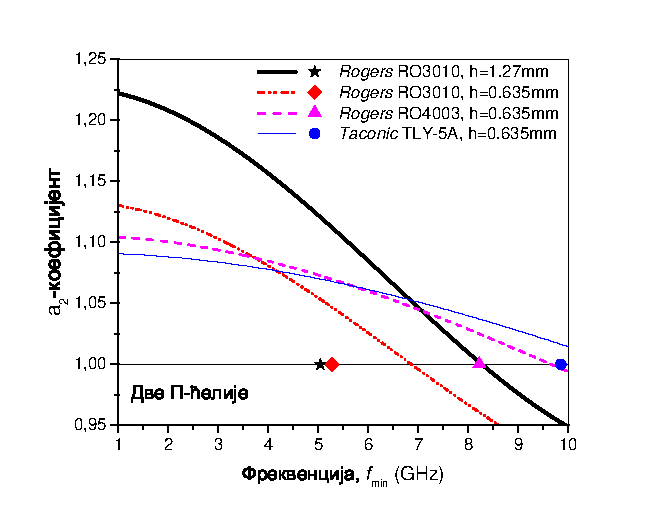
\includegraphics[width=0.8\textwidth]{sl_ekv/fig4b}
\label{f4b}}
\caption{Поређење коефицијената $a$ за еквивалентну шему са (а) једном (б) две П-ћелије за случај са \Fig{f3a}. Хоризонталне црне линије означавају вредност 1 на вертикалној оси, а маркери означавају фреквенције минимума $S_{11}$ за одговарајуће супстрате. За $k_m \in \mathbb{R}$ потребно је $a_{1,2}>1$.}
\label{f4}
\end{figure}
%%%%%%%%%%%%%%%%%%%%%%%%%%%%%%%%%%%%%%%%%%%%%%%%%%%%%%%%%%%%%%%%%%%%%%%%%%%%%%%%%%

3Д електромагнетне симулације и мерења за све структуре са \Fig{f3} показују да се минимум
$S_{11}$ јавља пре резонансе СРР-а, $f_r$, због чега је прва заграда у (2) негативна. Како би се добила реална вредност коефицијента спреге $k_m$, (која омогућава слагање фреквенција првог минимума $S_{11}$ добијених из еквивалентне шеме и симулације), неопходно је да десна страна једначине буде позитивна, што захтева $a_{1,2}>1$. 

На сл.~\ref{f4a} и \ref{f4b} приказано је поређење коефицијената $a$ израчунатих за шеме са једном и две ћелије, респективно, за СРР спрегнут са 50-омским микрострип водом [\Fig{f3a}] на различитим супстратима. На основу позиције минимума $S_{11}$ (одговарајући маркери), може се видети да услов $a>1$ није задовољен ни за један случај са \Fig{f4a}. С друге стране, услов је испуњен за све случајеве са \Fig{f4b}. Такође, супстрат са највећом пермитивношћу (Rogers RO3010) испољава најнижу горњу границу опсега у ком $k_m$ има реалну вредност (3.51 GHz за једну ћелију и 7.02 GHz за две). Треба приметити да коефицијент $a$ није функција параметара СРР-а, већ само фреквенције минимума $S_{11}$ и параметара вода.

Сл.~\ref{f4a} и \ref{f4b} јасно показују важну предност унапређеног модела структуре, у поређењу са шемом са једном П-ћелијом, а то је два пута већи опсег у ком $k_m$ има реалне вредности.

Уколико би уземљење преко вије било присутно, добио би се одзив пропусника опсега, и минимум $S_{11}$ би се појавио изнад трансмисионе нуле у симулацијама. У том случају, добро слагање може се добити помоћу шеме са једном ћелијом~\cite{bib16}. Тада би овде предложена шема била врло слична моделу пријављеном у~\cite{aznar_improved}, где је једна ћелија модификована како би се омогућило централно позиционирање индуктивности вије.

%%%%%%%%%%%%%%%%%%%%%%%%%%%%%%%%%%%%%%%%%%%%%%%%%%%%%%%%%%%%%%%%%%%%%%%%%%%%%%%%%%%%%
\subsubsection{Минимум $S_{11}$ изнад резонансе}
%%%%%%%%%%%%%%%%%%%%%%%%%%%%%%%%%%%%%%%%%%%%%%%%%%%%%%%%%%%%%%%%%%%%%%%%%%%%%%%%%%%%%

Обе еквивалентне шеме са \Fig{f2} испољавају други минимум $S_{11}$ изнад резонантне фреквенције СРР-а, који се не појављује у симулацијама или мерењима. Овај спуриозни ефекат је последица апроксимације дистрибуираног кола помоћу елемената са концентрисаним параметрима. Како би се повећао опсег у коме се еквивалентна шема може користити, неопходно је потиснути овај минимум ка што већим фреквенцијама. Ово се постиже коришћењем шеме са две ћелије.

Како би се разјаснио овај ефекат, почиње се од услова за идеално прилагођење (минимум $S_{11}$) за симетрично коло (следећи Бартлетову теоерему): $Y_\text{in,even} Y_\text{in,odd}=Y_0^2$, где се парна и непарна адмитанса одређују постављањем отворене везе, односно кратког споја у раван симетрије. После преуређења, услов се може преформулисати као
\begin{equation}
\frac{\omega_r^2 - \omega_\text{min}^2}{\omega_r^2-(1-k_m^2)\omega_\text{min}^2} =
a_{1,2}^{-1}
\end{equation}
где вредности $a_{1,2}$ одговарају изразима (3) и (4) за једну и две ћелије, респективно. На ниским учестаностима $a_2$ може се апроксимирати као $a_2^{-1} \approx
\frac{L}{C} Y_0^2 + \frac{b}{2}$. Поређењем овог израза са (3) примећује се да је коефицијент уз члан $b$ четири пута мањи. Пошто је $b$ пропорционално квадрату учестаности [видети (4)], ово имплицира да $a_2$ варира двоструко спорије са учестаношћу него $a_1$, због чега испољава фреквенцијску зависност ближу очекиваној за идеални вод (који би требало да има константну вредност коефицијента $a$). 
\begin{figure}[!t]
\centering
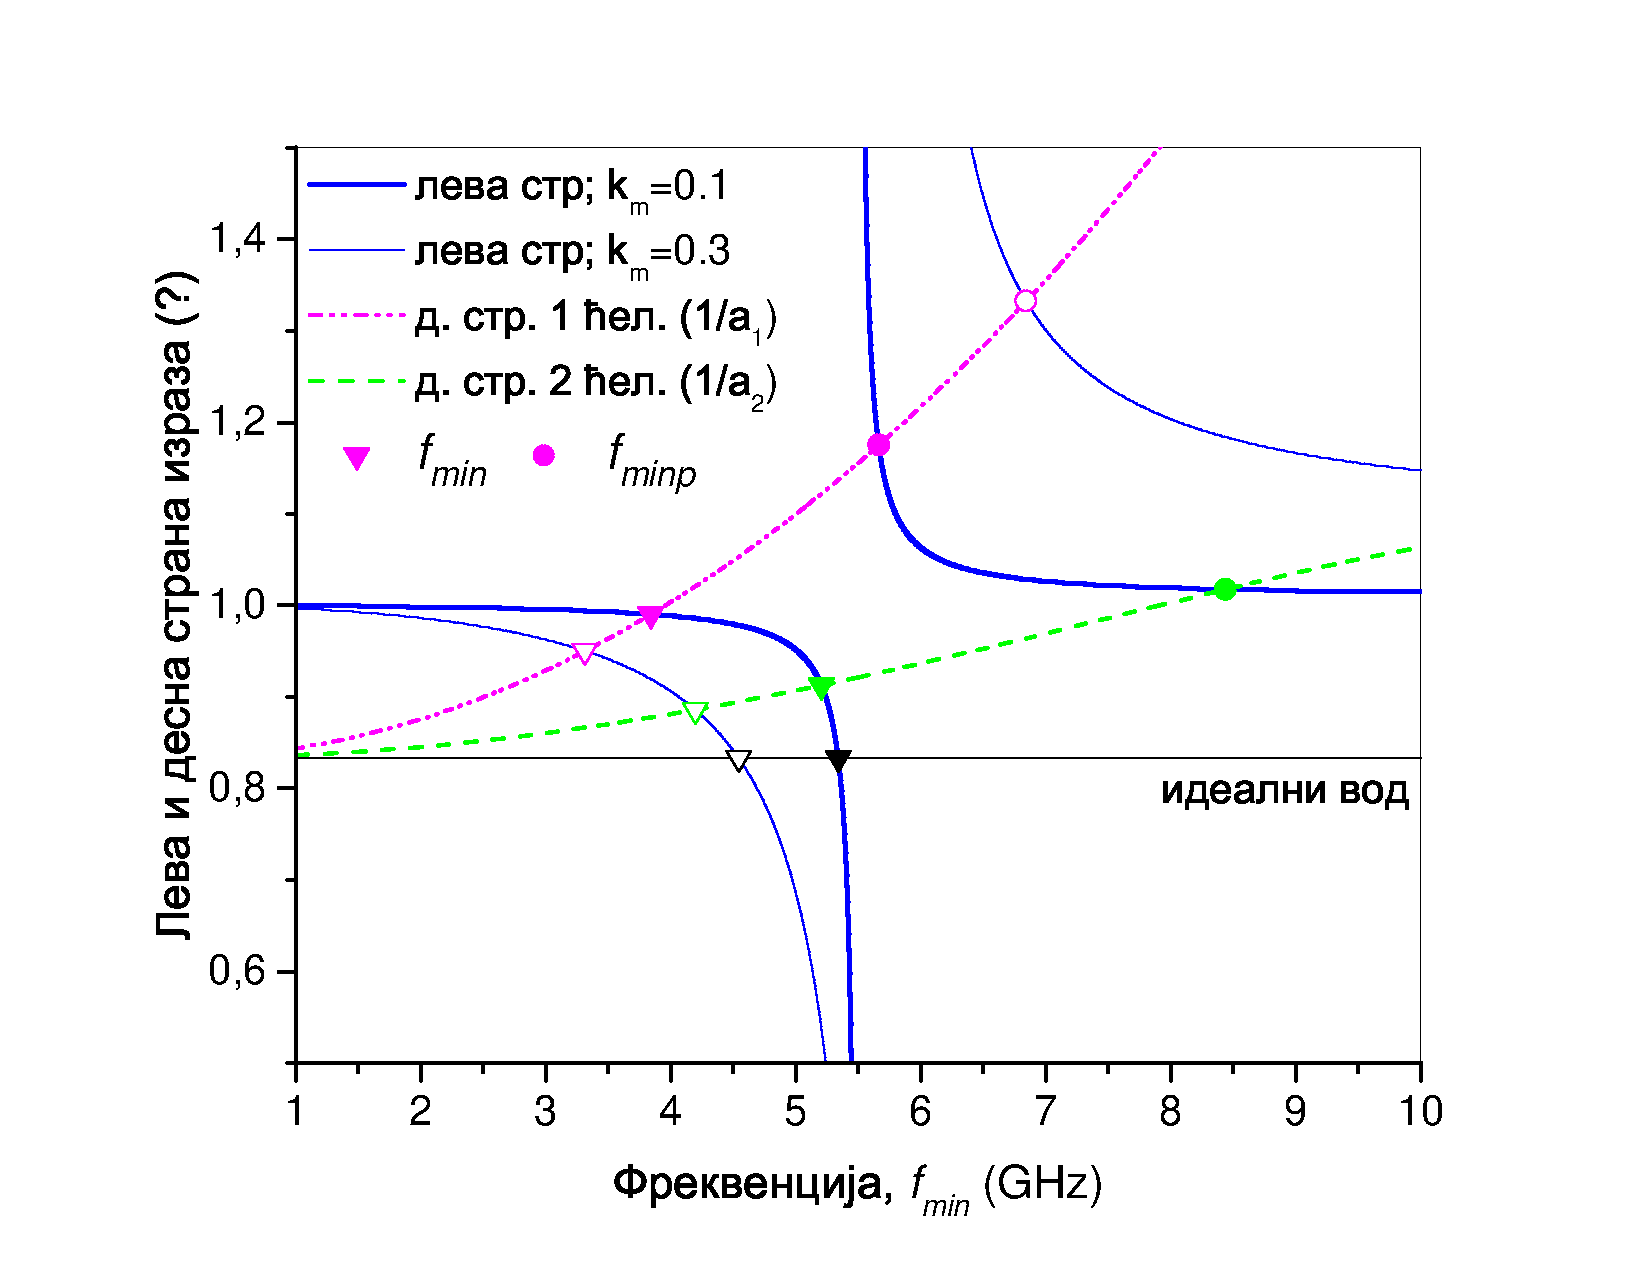
\includegraphics[width=\textwidth]{sl_ekv/fig5}
\caption{График зависности леве (пуне линије) и десне (испрекидане линије) стране израза (5). Тачке пресека представљају минимуме $S_{11}$ за одговарајуће случајеве.}
\label{f5}
\end{figure}

На \Fig{f5} лева и десна страна израза (5) су приказане на једну и две ћелије и за два различита коефицијента спреге (параметри вода одговарају случају са \Fig{f3a}). Пресечне тачке одговарајућих кривих за леву и десну страну означавају решења (5) и, према томе, минимуме $Ѕ_{11}$. Пресечне тачке испод резонансе СРР-а су означене троугловима, док су оне изнад, обележене круговима, паразитни минимуми $f_\text{minp}$, одсутни у симулацијама. Лева страна ове једначине не зависи од броја ћелија, већ само од коефицијента спреге $k_m$ и резонансе $f_r$ (пуне линије). Повећањем јачине спреге, ова крива се ,,шири`` (упоредити дебље и тање линије на слици), тако да је могуће подесити фреквенције оба минимума $Ѕ_{11}$ у датом опсегу. Такође, десна страна зависи само од параметара вода $L$ и $C$ (који су у основи одређени избором супстрата и карактеристичне импедансе), и има драстично другачији нагиб за основно и унапређено коло. Са слике се јасно види да је десна страна израза, која одговара унапређеном колу, много повољнија што се тиче паразитног минимума, који се јавља на много вишим фреквенцијама. Конкретно, за мале вредности коефицијента спреге ($k_m\sim 0.1$), други минимум $Ѕ_{11}$ јавља се одмах иза резонансе СРР-а за коло са једном ћелијом, чиме се драстично смањује његов фреквенцијски опсег.

%%%%%%%%%%%%%%%%%%%%%%%%%%%%%%%%%%%%%%%%%%%%%%%%%%%%%%%%%%%%%%%%%%%%%%%%%%%%%%%%%%%%%
\subsubsection{Екстраховани параметри еквивалентног кола}
%%%%%%%%%%%%%%%%%%%%%%%%%%%%%%%%%%%%%%%%%%%%%%%%%%%%%%%%%%%%%%%%%%%%%%%%%%%%%%%%%%%%%

Екстраховани параметри за коло са две ћелије [\Fig{f3f}] дати су у табели~\ref{tab2} за све конфигурације са \Fig{f3}.
\begin{table}[!t]
% increase table row spacing, adjust to taste
\renewcommand{\arraystretch}{1.3}
% if using array.sty, it might be a good idea to tweak the value of
% \extrarowheight as needed to properly center the text within the cells
\caption{Екстраховани параметри за кофигурације са \Fig{f3}.}
\label{tab2}
\centering
% Some packages, such as MDW tools, offer better commands for making tables
% than the plain LaTeX2e tabular which is used here.
\begin{tabular}{|l|c|c|c|c|c|}
\hline
модел & $f_r$(GHz) & $f_\text{min}$(GHz) & $C$(pF) & $C_S$(pF) & $k_m$ \\
\hline
\Fig{f3a} & 5.47 & 5.04 & 0.72 & 0.107 & 0.14 \\
\hline
\Fig{f3b} & 5.48 & 5.14 & 0.82 & 0.106 & 0.167 \\
\hline
\Fig{f3c} & 6.19 & 4.84 & 0.74 & 0.084 & 0.28 \\
\hline
\Fig{f3d} & 6.14 & 4.72 & 0.86 & 0.088 & 0.41 \\
\hline
\end{tabular}
\end{table}
Разлика у $C_S$ је услед другачијих резонантних учестаности, у складу са (1). Коефицијент спреге $k_m$ више варира, и значајно је већи за структуре без процепа у најближој ивици, где је спрега најизраженија. 

\subsection{\label{sec:ML2SP}
Микрострип вод спрегнут са два СРР-а са асиметричним процепима}
\begin{figure}[!t]
    \subfloat[]{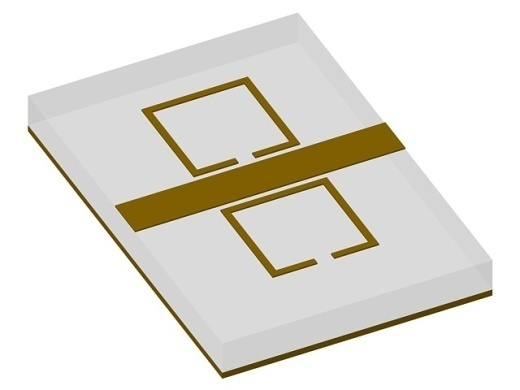
\includegraphics[width=0.48\columnwidth]{sl_ekv/fig6a}
\label{f6a}}
\subfloat[]{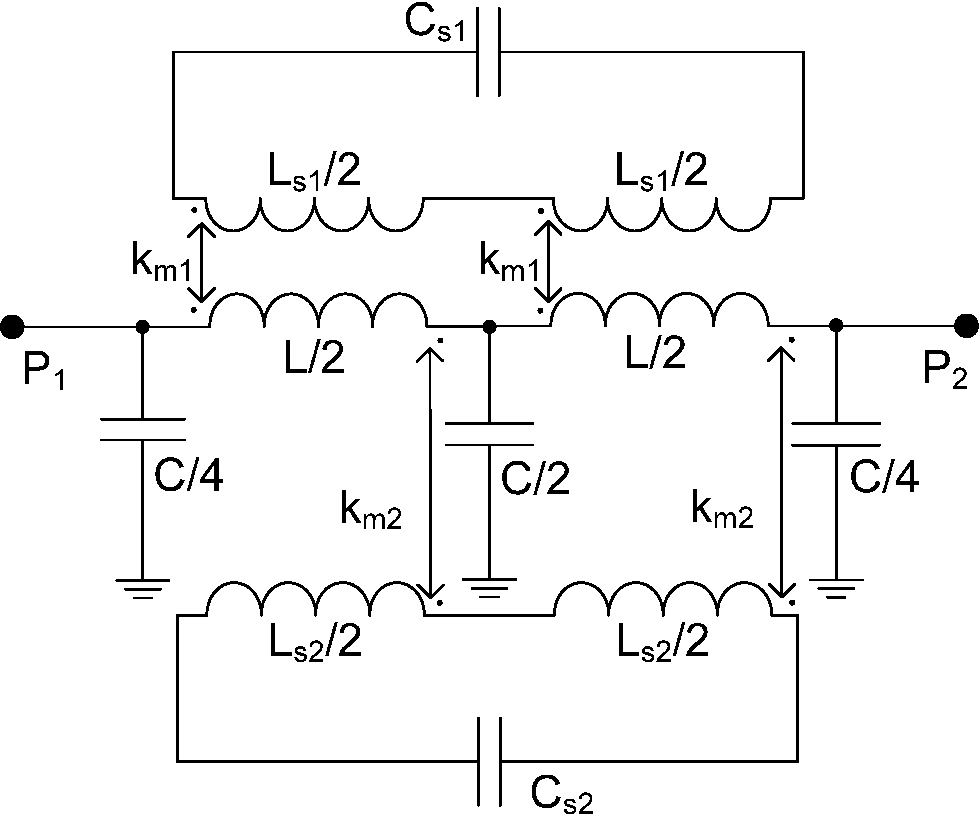
\includegraphics[width=0.48\columnwidth]{sl_ekv/fig6b}
\label{f6b}}
\caption{(a) Микрострип вод спрегнут са два СРР-а са асиметричним процепима и (б) одговарајућа еквивалентна шема.}
\label{f6}
\end{figure}
Микрострипи вод са два асиметрична СРР-а, где је један процеп на ближој а други на даљој ивици [\Fig{f6a}] има компликованију еквивалентну шему [\Fig{f6b}] него у претходном случају. Она је суперпозиција две шеме са \Fig{f3f}, зато што СРР-ови имају различите спреге и резонантне фреквенције. 

Вредности екстрахованих параметара $C_{s1}=0.105\, \mathrm{pF}$ и $C_{s2}=0.081\,
\mathrm{pF}$ одређене су на основу резонантних фреквенција $f_{r1}$ и $f_{r2}$, добијених симулацијом.

Коефицијент магнетне спреге $k_{m1,2}$  одређен је применом Бартлетове теореме на коло са \Fig{f6b}, на сличан начин као и за \Fig{f2b}. Да би се добили $k_{m1,2}$ треба решити следећи систем (пошто постоје два минимума $S_{11}$, $f_\text{min1,2}$):
\begin{equation}
\begin{split}
\frac{\omega_\text{min1}^2}{\omega_{r1}^2-\omega_\text{min1}^2}k_{m1}^2 +
\frac{\omega_\text{min1}^2}{\omega_{r2}^2-\omega_\text{min1}^2}k_{m2}^2 = & a_2^{(1)} -1, \\
\frac{\omega_\text{min2}^2}{\omega_{r1}^2-\omega_\text{min2}^2}k_{m1}^2 +
\frac{\omega_\text{min2}^2}{\omega_{r2}^2-\omega_\text{min2}^2}k_{m2}^2 = & a_2^{(2)} -1;
\end{split}
\end{equation}
где су $a_2^{(1),(2)}$ израчунати на основу (4). Коначно, добија се $k_{m1}=0.14$ и $k_{m2}=0.26$.

За еквивалентну шему са једном ћелијом, систем (6) остаје исти, осим што је потребно заменити $a_2$ са $a_1$, израчунатим на основу (3). У том случају, прва једначина у (6) одговара првом минимуму $S_{11}$ испод резонансе. Дакле, коефицијенти на левој страни биће позитивни, док је десна страна негативна, па једначина нема решења. Последично, немогуће је поклопити први минимум у симулацији/мерењу и еквивалентној шеми. Други минимум, међутим, налази се између резонанси, зато је један од коефицијената на левој страни (6) негативан, па је могуће извршити поклапање. Онда важи следећа релација између коефицијената спреге:
\begin{equation}
k_{m1}^2 = \left(\omega_\text{min2}^2-\omega_{r1}^2 \right) \left(\frac{k_{m2}^2}{\omega_{r2}^2-\omega_\text{min2}^2 } - \frac{a_1^{(2)}-1}{\omega_\text{min2}^2}\right).
\end{equation}
При решавању (7), треба узети у обзир да $k_{m2}$
(који одговара СРР-у са даљим процепом) треба бити веће од $k_{m1}$. 

\subsection{\label{sec:ML2SPerp} 
Микрострип вод спрегнут са СРР-овима са нормалним процепима}
%%%%%%%%%%%%%%%%%%%%%%%%%%%%%%%%%%%%%%%%%%%%%%%%%%%%%%%%%%%%%%%%%%%%%%%%%%%%%
\begin{figure}[!t]
\centering
\subfloat[]{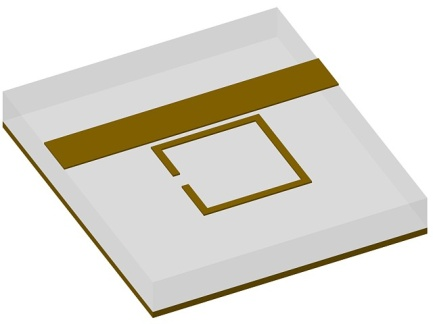
\includegraphics[width=0.4\columnwidth]{sl_ekv/fig7a}
\label{f7a}}\hfil
\subfloat[]{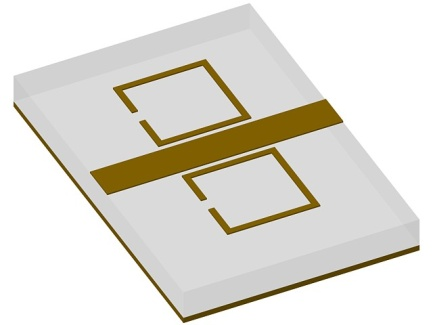
\includegraphics[width=0.4\columnwidth]{sl_ekv/fig7b}
\label{f7b}}\\
\subfloat[]{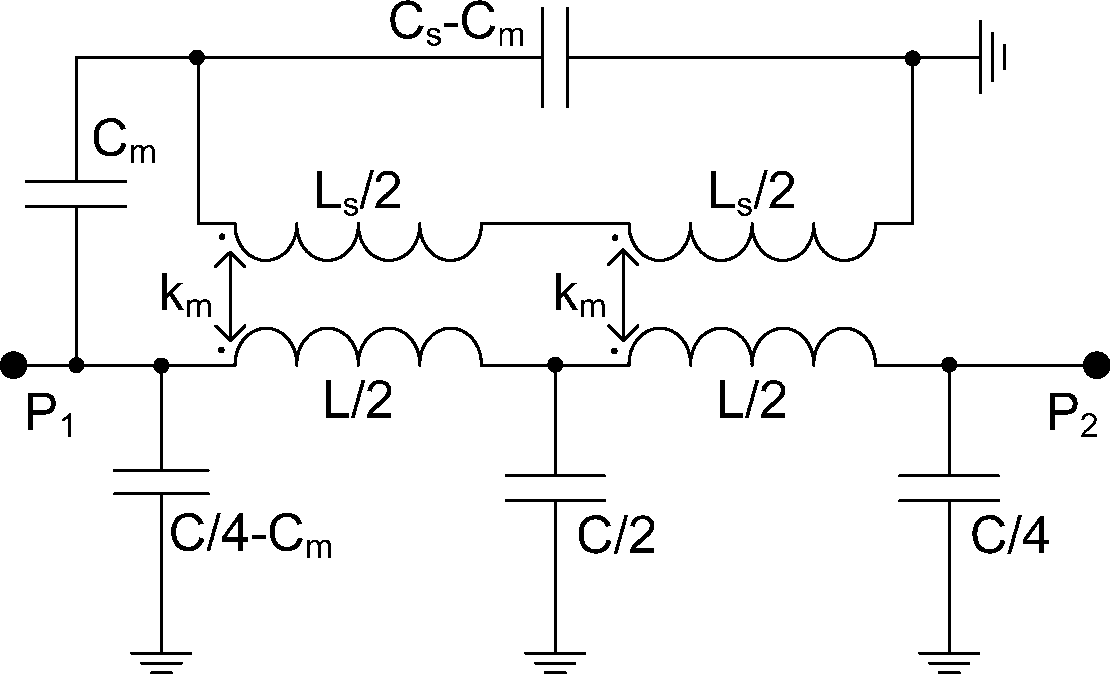
\includegraphics[width=0.6\columnwidth]{sl_ekv/fig7c}
\label{f7c}}
\caption{СРР-ови са процепима нормалним у односу на вод: (а) један СРР,
(б) два СРР-а симетрично у односу на вод; оба случаја се могу моделовати истим еквивалентними колом (в).} 
\label{f7}
\end{figure}
%%%%%%%%%%%%%%%%%%%%%%%%%%%%%%%%%%%%%%%%%%%%%%%%%%%%%%%%%%%%%%%%%%%%%%%%%%%%%
СРР-ови приказани на \Fig{f7} разликују се од претходних конфигурација, утолико што су заротирани за 90 степени, што значи да цела структура више није симетрична у односу на микрострип вод. У овом случају, електрично поље вода паралелно је у односу на процеп, што узрокује додатну електричну спрегу, укључену у еквивалентну шему приказану на \Fig{f7c}.

Микрострип вод, оптерећен са једним СРР-ом са нормалним процепом [\Fig{f7a}], има исту еквивалентну шему као и два СРР-а симетрично постављена с обе стране [\Fig{f7b}], само са различитим вредностима параметара.

Вредности одговарајућих елемената кола $L$, $C$ и $L_S$ дате су у табели~\ref{tab1} за конфигурације са \Fig{f7}. Коефицијент магнетне спреге $k_m$ за структуре са сл.~\ref{f7a} и \ref{f7b} апроксимиране су вредностима добијеним за одговарајуће СРР-ове са процепима паралелним и даље од вода [\Fig{f3c} и \ref{f3d}, респективно], пошто они имају веома сличну расподелу струје. Преостали параметри, $C_S$ и $C_m$, су одређени коришћењем резонантне учестаности ($C_S$ се добија као функција од $C_m$, које се изводи помоћу процедуре фитовања са симулацијом).

%%%%%%%%%%%%%%%%%%%%%%%%%%%%%%%%%%%%%%%%%%%%%%%%%%%%%%%%%%%%%%%%%%%%%%%%%%%%%%
\begin{figure}[!t]
\centering
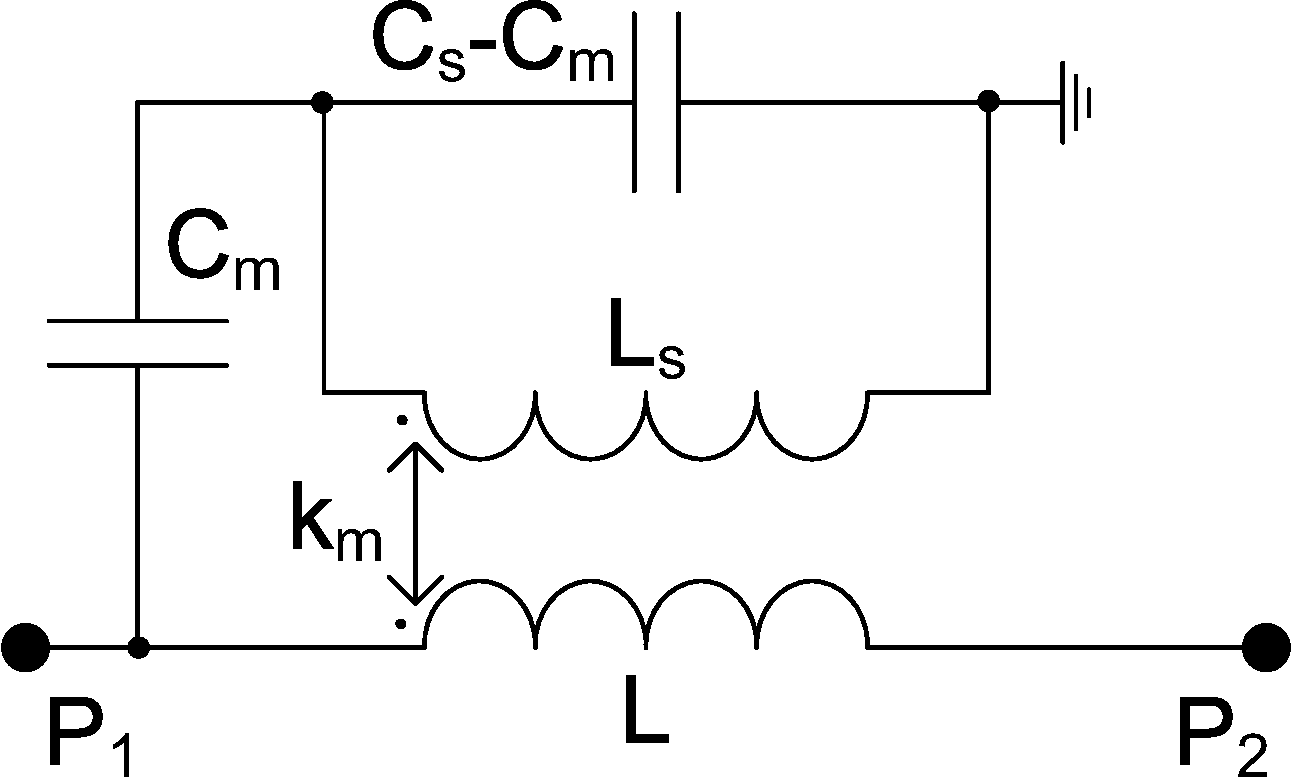
\includegraphics[width=0.4\columnwidth]{sl_ekv/fig8}
\caption{Поједностављена шема за рачунање резонантне учестаности.}
\label{f8}
\end{figure}
%%%%%%%%%%%%%%%%%%%%%%%%%%%%%%%%%%%%%%%%%%%%%%%%%%%%%%%%%%%%%%%%%%%%%%%%%%%%%%
Како би се одредила приближна резонантна фреквиенција (односно минимум $Ѕ_{21}$), биће коришћена шема са \Fig{f8}, на којој су паралелно везани кондензатори уклоњени, у поређењу са \Fig{f7c}. Ово значајно олакшава анализу, док је утицај на резонансу занемарљив.

Исписивањем система једначина на основу Кирхофових закона, добија се следећа матрична релација између струја и напона на портовима 1 и 2:
\begin{multline}\label{mat8}
\begin{bmatrix}
j\omega (1-L_S/L_m) & 1 \\
\dfrac{j}{\omega L_m}(1-\omega^2 L_S C_S) + j\omega C_m & 0
\end{bmatrix}
\begin{bmatrix} V_1 \\ I_1 \end{bmatrix}  \\  = 
\begin{bmatrix}
-j\omega C_m L_S/L_m & 1 - \omega^2 L_m C_m (1/k_m^2 -1) \\
\dfrac{j}{\omega L_m}(1-\omega^2 L_S C_S) & \dfrac{L}{L_m}(1-\omega^2 L_S C_S(1-k_m^2))
\end{bmatrix}
\begin{bmatrix} V_2 \\ I_2 \end{bmatrix}\;.
\end{multline}
Услов за резонансу, односно непостојање трансмисије између портова, може се преформулисати као захтев да имамо нетривијално решење на левој страни, када је $V_2,I_2=0$ (тј. десна страна је једнака нули), што може бити испуњено само ако је детерминанта матрице на левој страни једнака нули:
\begin{equation}
\frac{j}{\omega L_m}(1-\omega^2 L_S C_S) + j\omega C_m
= \frac{j}{\omega L_m}(1-\omega^2 L_S C_S+\omega^2 L_m C_m)=0
\end{equation}
што даје следећу резонантну фреквенцију:
\begin{equation}
f_r = \frac{1}{2\pi\sqrt{L_S C_S - L_mC_m}} 
\end{equation}
са $L_m=k_m\sqrt{LL_S}$. 
Може се показати да, услед реципрочности ($S_{12}=S_{21}$), матрице на левој и десној страни (\ref{mat8}) једнаке, али у овом случају је једноставније разматрати ону на левој страни.

\begin{table}[!t]
% increase table row spacing, adjust to taste
\renewcommand{\arraystretch}{1.3}
% if using array.sty, it might be a good idea to tweak the value of
% \extrarowheight as needed to properly center the text within the cells
\caption{Екстраховани параметри за конфигурације са \Fig{f7}.}
\label{tab3}
\centering
% Some packages, such as MDW tools, offer better commands for making tables
% than the plain LaTeX2e tabular which is used here.
\begin{tabular}{|l|c|c|c|c|c|}
\hline
Конфигурације & $f_r$(GHz) & $C$(pF) & $C_S$(pF) & $k_m$ & $C_m$(pF) \\
\hline
\Fig{f7a} & 5.8 & \textbf{0.74} & 0.102 & \textbf{0.29} & \textbf{0.055} \\
\hline
\Fig{f7b} & 5.86 & \textbf{0.86} & 0.108 & \textbf{0.42} & \textbf{0.08} \\
\hline
\end{tabular}
\end{table}
Екстраховане вредности елемената кола (табела~\ref{tab3}) добијене су после мале оптимизације параметара $C_s$, $C_m$ и $k_m$, потребне због анализе поједностављеног кола. Може се видети да су вредности $L$, $C_s$ и $L_s$ веома сличне за обе структуре, док се $C$, $C_m$ и $k_m$ разликују. Разлика у $C_m$ и $k_m$ последица је јаче спреге са два СРР-а.

%%%%%%%%%%%%%%%%%%%%%%%%%%%%%%%%%%%%%%%%%%%%%%%%%%%%%%%%%%%%%%%%%%%%%%%%%%%%%%%%%
\subsection{Каскадиране структуре}
%%%%%%%%%%%%%%%%%%%%%%%%%%%%%%%%%%%%%%%%%%%%%%%%%%%%%%%%%%%%%%%%%%%%%%%%%%%%%%%%%

%%%%%%%%%%%%%%%%%%%%%%%%%%%%%%%%%%%%%%%%%%%%%%%%%%%%%%%%%%%%%%%%%%%%%%%%%%%%%%%%%
\begin{figure}[!t]\centering
    \subfloat[]{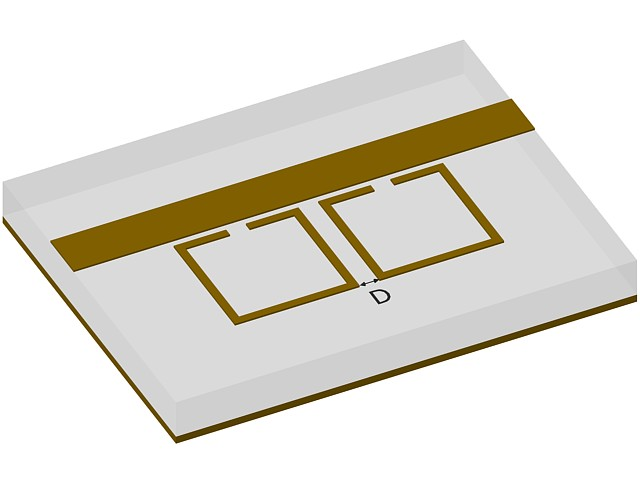
\includegraphics[width=0.55\columnwidth]{sl_ekv/k2.jpeg}
\label{fka}}\\
\subfloat[]{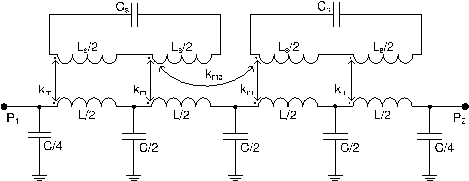
\includegraphics[width=0.9\columnwidth]{sl_ekv/kaskada}
\label{fkb}}
\caption{(a) Каскадирани СРР-ови (б) одговарајуће еквивалентно коло.}
\label{fk}
\end{figure}
%%%%%%%%%%%%%%%%%%%%%%%%%%%%%%%%%%%%%%%%%%%%%%%%%%%%%%%%%%%%%%%%%%%%%%%%%%%%%%%%%
Јединичне ћелије, разматране горе, могу се каскадирати како би се добили филтри са унапређеним опсегом, као што је приказано на \Fig{fka} за СРР-ове са процепом паралелним и близу вода. Ова структуре се моделује еквивалентним колом са \Fig{fkb}, са претходно екстрахованим параметрима, и додатном спрегом између резонатора, која се одређује из симулације два резонатора, и може се користити за моделовање произвољног броја спрегнутих СРР-ова, све док се спрега између несуседних елемената може занемарити. Добијени коефицијенти спреге $k_{mc}$ за различита растојања између резонатора приказани су у табели~\ref{tabk}. 
%%%%%%%%%%%%%%%%%%%%%%%%%%%%%%%%%%%%%%%%%%%%%%%%%%%%%%%%%%%%%%%%%%%%%%%%%%%%%%%%%
\begin{table}[!t]
% increase table row spacing, adjust to taste
\renewcommand{\arraystretch}{1.3}
% if using array.sty, it might be a good idea to tweak the value of
% \extrarowheight as needed to properly center the text within the cells
\caption{Екстраховани коефицијент спреге између резонатора, $k_{mc}$.}
\label{tabk}
\centering
% Some packages, such as MDW tools, offer better commands for making tables
% than the plain LaTeX2e tabular which is used here.
\begin{tabular}{|l|c|c|c|c|c|}
\hline
$D$ (mm) & 0.1 & 0.2 & 0.3 & 0.4 & 0.5\\
\hline
$k_{mc}$ & 0.155 & 0.102 & 0.078 & 0.052 & 0.03\\
\hline
\end{tabular}
\end{table}
%%%%%%%%%%%%%%%%%%%%%%%%%%%%%%%%%%%%%%%%%%%%%%%%%%%%%%%%%%%%%%%%%%%%%%%%%%%%%%%%%

%%%%%%%%%%%%%%%%%%%%%%%%%%%%%%%%%%%%%%%%%%%%%%%%%%%%%%%%%%%%%%%%%%%%%%%%%%%%%%%%%
\section{Валидација модела и резултати}
%%%%%%%%%%%%%%%%%%%%%%%%%%%%%%%%%%%%%%%%%%%%%%%%%%%%%%%%%%%%%%%%%%%%%%%%%%%%%%%%%

%%%%%%%%%%%%%%%%%%%%%%%%%%%%%%%%%%%%%%%%%%%%%%%%%%%%%%%%%%%%%%%%%%%%%%%%%%%%%%%%%
\begin{figure}[!t]
\centering
\subfloat[]{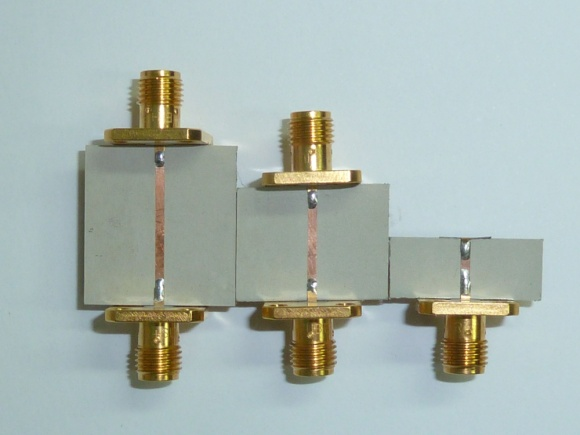
\includegraphics[width=0.4\columnwidth]{sl_ekv/fig9a}
\label{f9a}}\hfill
\subfloat[]{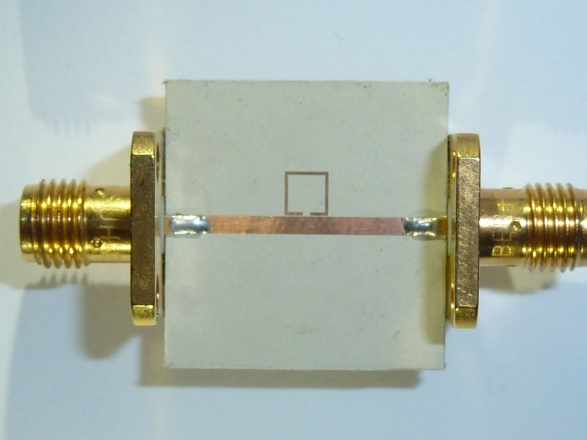
\includegraphics[width=0.4\columnwidth]{sl_ekv/fig9b}
\label{f9b}}
\caption{(a) Фабриковани наменски пројектовани LRL калибрациони сет за мерење $S$-параметара на референтним равнима и (б) микрострип вод оптерећен СРР-ом са паралелним процепом ближе воду.} 
\label{f9}
\end{figure}
%%%%%%%%%%%%%%%%%%%%%%%%%%%%%%%%%%%%%%%%%%%%%%%%%%%%%%%%%%%%%%%%%%%%%%%%%%%%%%%%%
Како би се валидирали предложени еквивалентни модели и екстракција њихових параметара, биће упоређене магнитуде и фазе $Ѕ$-параметара добијених мерењем, симулацијама и на основу еквивалентних шема. Симулације су вршене коришћењем идеализованих материјала без губитака, пошто и еквивалентне шеме не укључују губитке. Ипак, одређени губици у симулацијама и мерењима су ипак присутни услед зрачења. Наравно, мерења укључују и губитке у металима и диелектрицима. Све структуре су симулиране у програму WIPL-D~[wipl], и резултати су деембедовани на референтним равнима, означеним на \Fig{f1}. Измерени $Ѕ$-параметри су такође деембедовани на референтним равнима коришћењем LRL (Line-Reflect-Line) калибрационог сета приказаног на \Fig{f9a}, на анализатору мрежа Anritsu ME7838A. Фабриковани прототип микрострип вода оптерећеног са једним СРР-ом са паралелним процепом ближе воду приказан је на \Fig{f9b}.

%%%%%%%%%%%%%%%%%%%%%%%%%%%%%%%%%%%%%%%%%%%%%%%%%%%%%%%%%%%%%%%%%%%%%%%%%%%%%%%%%
\subsection{СРР-ови са паралелним процепом}
%%%%%%%%%%%%%%%%%%%%%%%%%%%%%%%%%%%%%%%%%%%%%%%%%%%%%%%%%%%%%%%%%%%%%%%%%%%%%%%%%

%%%%%%%%%%%%%%%%%%%%%%%%%%%%%%%%%%%%%%%%%%%%%%%%%%%%%%%%%%%%%%%%%%%%%%%%%%%%%%%%%
\begin{figure}[!t]
\centering
\subfloat[]{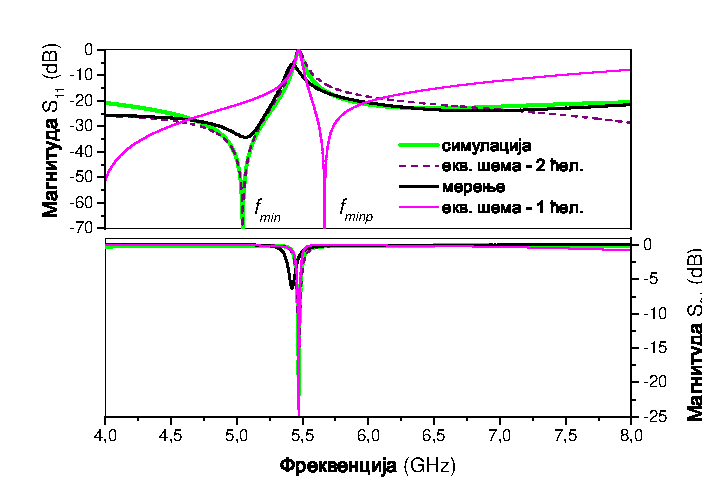
\includegraphics[width=\SirB]{sl_ekv/fig10a}
\label{f10a}}\\
\subfloat[]{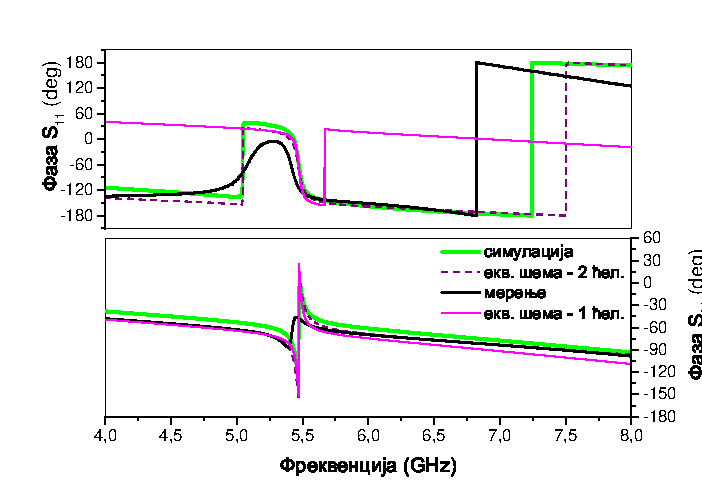
\includegraphics[width=\SirB]{sl_ekv/fig10b}
\label{f10b}}
\caption{Поређење магнитуда (а) и фаза (б) за $Ѕ$-параметре добијене мерењем, симулацијом и на основу еквивалентне шеме са једном и две П-ћелије за конфигурацију са \Fig{f3a}.}\label{f10}
\end{figure}
%%%%%%%%%%%%%%%%%%%%%%%%%%%%%%%%%%%%%%%%%%%%%%%%%%%%%%%%%%%%%%%%%%%%%%%%%%%%%%%%%
%%%%%%%%%%%%%%%%%%%%%%%%%%%%%%%%%%%%%%%%%%%%%%%%%%%%%%%%%%%%%%%%%%%%%%%%%%%%%%%%%
\begin{figure}[!t]
\centering
\subfloat[]{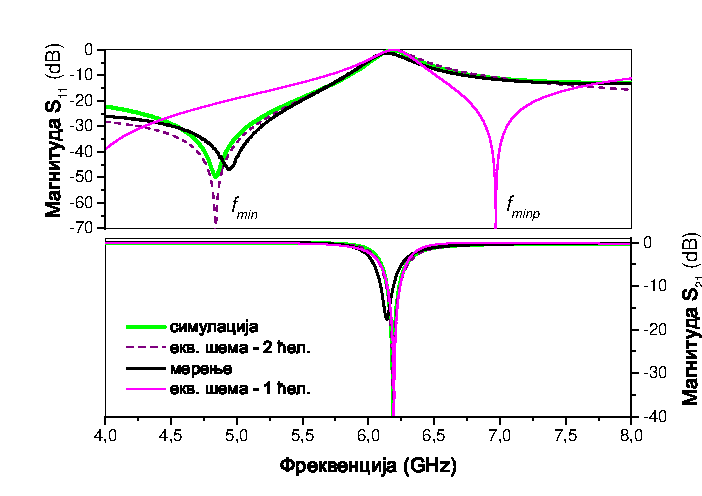
\includegraphics[width=\SirB]{sl_ekv/fig11a}
\label{f11a}}\\
\subfloat[]{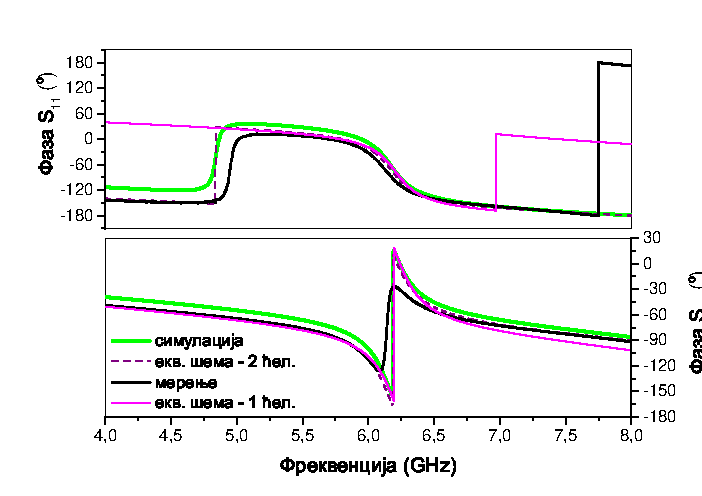
\includegraphics[width=\SirB]{sl_ekv/fig11b}
\label{f11b}}
\caption{Поређење магнитуда (а) и фаза (б) за $Ѕ$-параметре добијене мерењем, симулацијом и на основу еквивалентне шеме са једном и две П-ћелије за конфигурацију са \Fig{f3c}.} 
\label{f11}
\end{figure}
%%%%%%%%%%%%%%%%%%%%%%%%%%%%%%%%%%%%%%%%%%%%%%%%%%%%%%%%%%%%%%%%%%%%%%%%%%%%%%%%%

Резултати добијени мерењем, симулацијом и анализом помоћу еквивалентне шеме коришћењем две П-ћелије [\Fig{f3f}] за структуре са сл.~\ref{f3a} и \ref{f3c} приказане су на сл.~\ref{f10} и~\ref{f11}, респективно. Резултати се међусобно добро слажу у целом опсегу од 4 до 8 GHz. Мања одступања у магнитуди између еквивалентне шеме и мерења на \Fig{f10} налазе се на крају опсега, и могу се приписати присуству паразитног минимума $S_{11}$. Фреквенција овог минимума је око $8.8\,$GHz услед релативно слабе спреге (упоредити са \Fig{f5}). Насупрот томе, резултати добијени са еквивалентном шемом која користи једну ћелију [\Fig{f3e}] показују велико неслагање са симулацијама и мерењима, без обзира на вредност $k_m$. Заправо, овај поједностављени модел је тачан само на резонантној учестаности и у непосредној околини. Први минимум $S_{11}$ јавља се на далеко нижој учестаности од измерене, и није могуће преклопити их за било коју реалну вредност $k_m$, у складу са~(3). Коефицијенти спреге за еквивалентну шему са једном ћелијом добијени су поступком фитовања и њихове вредности су $k_m=0.1$ за \Fig{f10} и $k_m=0.23$ за \Fig{f11}, за СРР са процепом даље од вода.

%\begin{figure}[!t]
%\centering
%\subfloat[]{\includegraphics[width=0.48\columnwidth]{fig12a}
%\label{f12a}}\hfill
%\subfloat[]{\includegraphics[width=0.48\columnwidth]{fig12b}
%\label{f12b}}
%\caption{Comparison of magnitudes (a) and phases (b) of $S$-parameters obtained by full-wave
%simulations and equivalent circuit analysis with one and two $\Pi$-cells for the configuration
%in \Fig{f3b}.}
%\label{f12}
%\end{figure}
%\sout{To demonstrate that the same two-cells equivalent circuit [\Fig{f3f}] can be used to
%model the microstrip line loaded with two SRRs [\Fig{f3b}] we compare the results given by a
%full-wave simulation and equivalent circuit model in \Fig{f12}. The discrepancy at the end of
%the band is caused again by the presence of the second SRR resonance. Once more, the circuit
%with one cell is unable to achieve good matching over a wide frequency band, being accurate
%only around the resonance. In this last model, the value of magnetic coupling obtained by
%fitting is $k_m=0.135$.}

%%%%%%%%%%%%%%%%%%%%%%%%%%%%%%%%%%%%%%%%%%%%%%%%%%%%%%%%%%%%%%%%%%%%%%%%%%
\subsection{Микрострип вод са два СРР-а са асиметричним процепима}
%%%%%%%%%%%%%%%%%%%%%%%%%%%%%%%%%%%%%%%%%%%%%%%%%%%%%%%%%%%%%%%%%%%%%%%%%%

%%%%%%%%%%%%%%%%%%%%%%%%%%%%%%%%%%%%%%%%%%%%%%%%%%%%%%%%%%%%%%%%%%%%%%%%%%
\begin{figure}[!t]
\centering
\subfloat[]{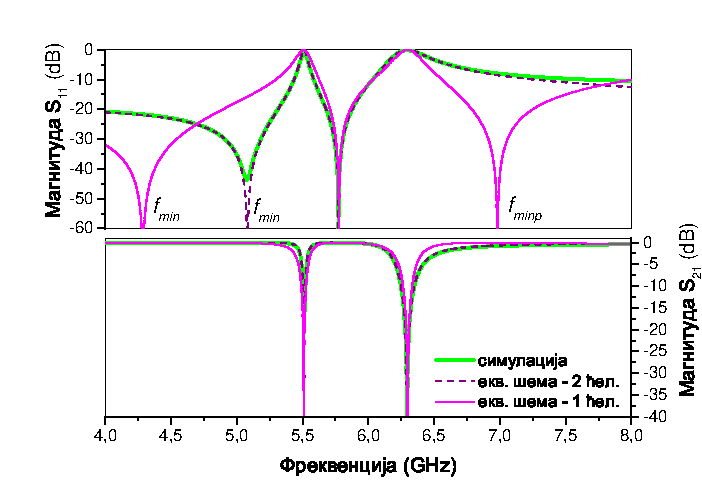
\includegraphics[width=\SirB]{sl_ekv/fig13a}
\label{f13a}}\\
\subfloat[]{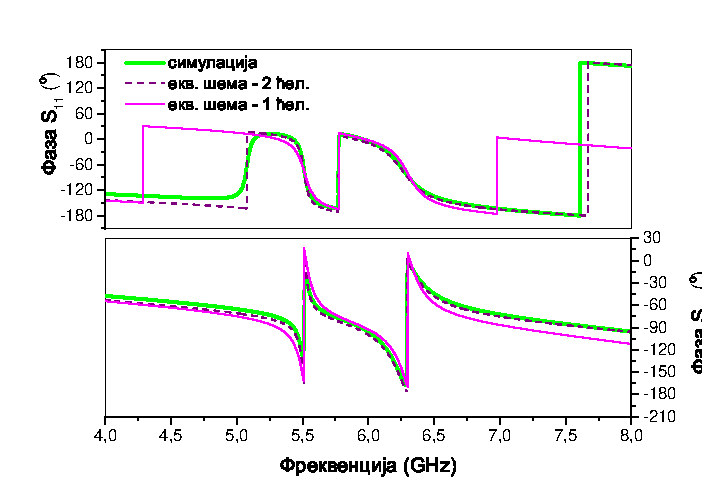
\includegraphics[width=\SirB]{sl_ekv/fig13b}
\label{f13b}}
\caption{Поређење магнитуда (а) и фаза (б) за $Ѕ$-параметре добијене мерењем, симулацијом и на основу еквивалентне шеме са једном и две П-ћелије за конфигурацију са \Fig{f6a}.} 
\label{f13}
\end{figure}
%%%%%%%%%%%%%%%%%%%%%%%%%%%%%%%%%%%%%%%%%%%%%%%%%%%%%%%%%%%%%%%%%%%%%%%%%%
Поређење између симулације и еквивалентне шеме са једном и две ћелије, за микрострип вод оптерећен са два СРР-а са асиметричним процепима (један ближе воду, други даље од њега), дато је на \Fig{f13}. За случај са шеме са две ћелије, може се видети скоро савршено слагање, и у магнитуди и у фази, у целом опсегу од 4 до 8 GHz. 

За коло са једном ћелијом, добро поклапање се добија само око другог минимума, за коефицијенте спреге $k_{m1}=0.16$ и $k_{m2}=0.18$, што није очекивано, с обзиром да су спрегнуте гране СРР-ова веома различите (са и без процепа). Може се видети да је око друге резонансе неслагање не само у $Ѕ_{11}$, већ и у $Ѕ_{21}$, пошто није изводљиво померити трећи минимум ка вишој фреквенцији. Такође, први минимум $Ѕ_{11}$ није уопште могуће поклопити са колом са једном ћелијом, као што је предвиђено у секцији~\ref{sec3:2}. 

%%%%%%%%%%%%%%%%%%%%%%%%%%%%%%%%%%%%%%%%%%%%%%%%%%%%%%%%%%%%%%%%%%%%%%%%%%
\subsection{СРР-ови са нормалним процепом у односу на вод}
%%%%%%%%%%%%%%%%%%%%%%%%%%%%%%%%%%%%%%%%%%%%%%%%%%%%%%%%%%%%%%%%%%%%%%%%%%

%%%%%%%%%%%%%%%%%%%%%%%%%%%%%%%%%%%%%%%%%%%%%%%%%%%%%%%%%%%%%%%%%%%%%%%%%%
\begin{figure}[!t]
\centering
\subfloat[]{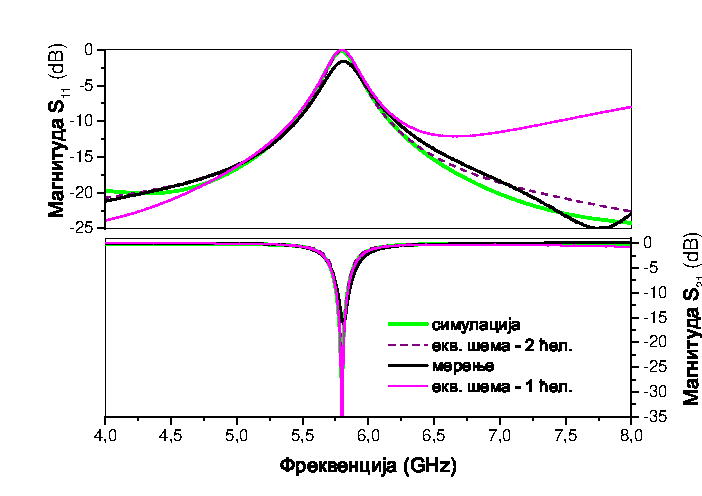
\includegraphics[width=\SirB]{sl_ekv/fig14a}
\label{f14a}}\\
\subfloat[]{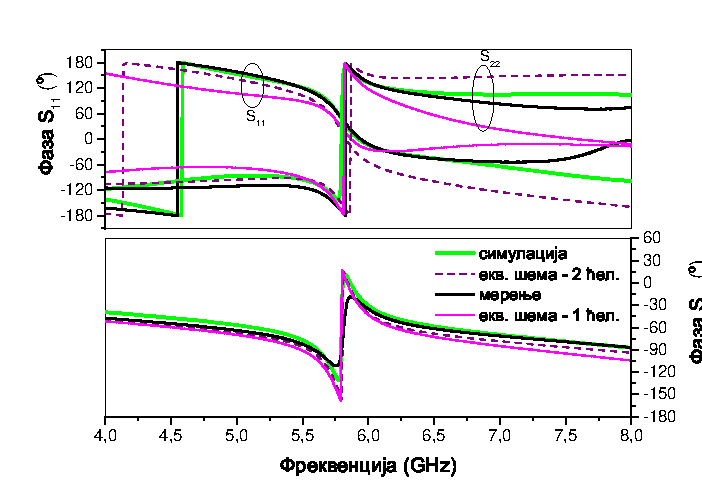
\includegraphics[width=\SirB]{sl_ekv/fig14b}
\label{f14b}}
\caption{Поређење магнитуда (а) и фаза (б) за $Ѕ$-параметре добијене мерењем, симулацијом и на основу еквивалентне шеме са једном и две П-ћелије за конфигурацију са \Fig{f7a}.}
\label{f14}
\end{figure}
%%%%%%%%%%%%%%%%%%%%%%%%%%%%%%%%%%%%%%%%%%%%%%%%%%%%%%%%%%%%%%%%%%%%%%%%%%
Како би се показале предности унапређене шеме [\Fig{f7c}] у односу на модел са једном ћелијом за СРР са нормалним процепом [\Fig{f7a}], на \Fig{f14} упоређене су магнитуде и фазе $Ѕ$-параметара добијених мерењем, симулацијом и еквивалентном шемом са једном и две П-ћелије. Још једном, резултати за две ћелије су у веома добром слагању са симулацијама и мерењима у целом опсегу од 4 до 8 GHz. Треба приметити да у овом случају не постоји минимум рефлексије испод резонансе СРР-а, као у случајевима са паралелним процепом. Иако је структура асиметрична, само магнитуда $Ѕ_{11}$ је приказана (разлика са $Ѕ_{22}$ је изражена само у фази). Еквивалентна шема са једном ћелијом се сада понаша много боље него у случајевима са паралелним процепом, али предложена шема са две ћелије је ипак боља у ширем опсегу. Екстраховани параметри за модел са једном ћелијом су $k_m=0.28$, $C_m=0.062\,\mathrm{pF}$.

%%%%%%%%%%%%%%%%%%%%%%%%%%%%%%%%%%%%%%%%%%%%%%%%%%%%%%%%%%%%%%%%%%%%%%%%%%
\begin{figure}[!t]
\centering
\subfloat[]{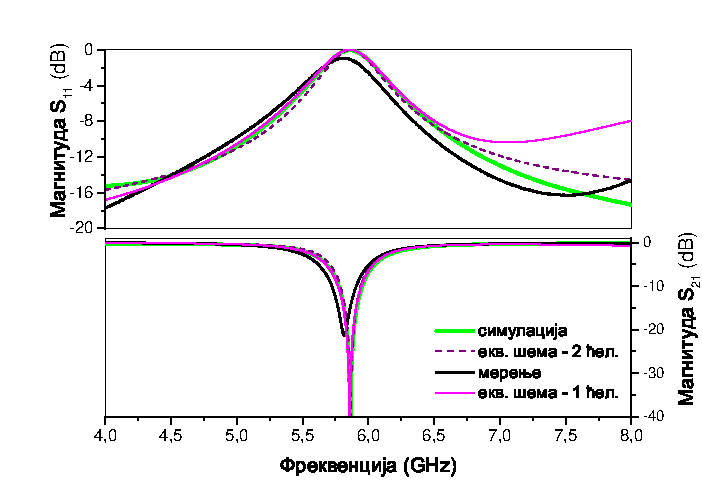
\includegraphics[width=\SirB]{sl_ekv/fig15a}
\label{f15a}}\\
\subfloat[]{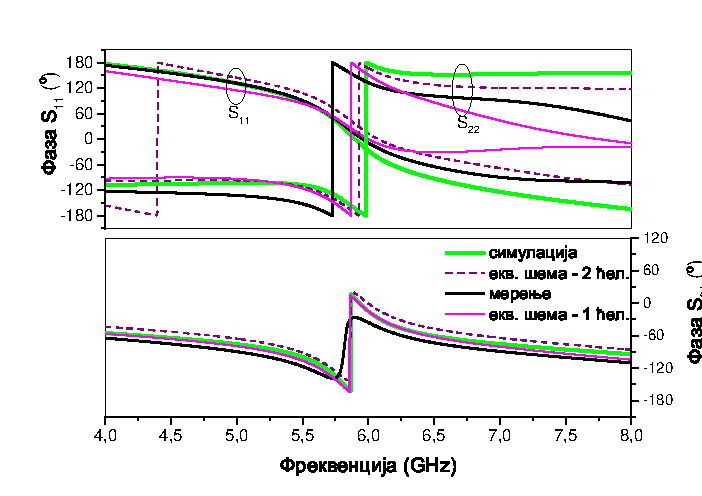
\includegraphics[width=\SirB]{sl_ekv/fig15b}
\label{f15b}}
\caption{Поређење магнитуда (а) и фаза (б) за $Ѕ$-параметре добијене мерењем, симулацијом и на основу еквивалентне шеме са једном и две П-ћелије за конфигурацију са \Fig{f7b}.}
\label{f15}
\end{figure}
%%%%%%%%%%%%%%%%%%%%%%%%%%%%%%%%%%%%%%%%%%%%%%%%%%%%%%%%%%%%%%%%%%%%%%%%%%
Резултати симулације и анализе помоћу еквивалентне шеме са једном и две П-ћелије за конфигурацију са \Fig{f7b} приказани су на \Fig{f15}. Резултати за две ћелије су у веома добром слагању са симулацијом. Модел са једном ћелијом одговара симулацији у ширем опсегу него у случају само једног СРР-а, и слагање је добро до \SI{7.5}{\giga\hertz}. Екстраховани параметри кола за шему са једном ћелијом су $k_m=0.39$ и $C_m=0.095\, \mathrm{pF}$.

%%%%%%%%%%%%%%%%%%%%%%%%%%%%%%%%%%%%%%%%%%%%%%%%%%%%%%%%%%%%%%%%%%%%%%%%%%
\subsection{Каскадирани СРР-ови са процепом паралелним воду}
%%%%%%%%%%%%%%%%%%%%%%%%%%%%%%%%%%%%%%%%%%%%%%%%%%%%%%%%%%%%%%%%%%%%%%%%%%

%%%%%%%%%%%%%%%%%%%%%%%%%%%%%%%%%%%%%%%%%%%%%%%%%%%%%%%%%%%%%%%%%%%%%%%%%%
\begin{figure}[!t]
\centering
\subfloat[]{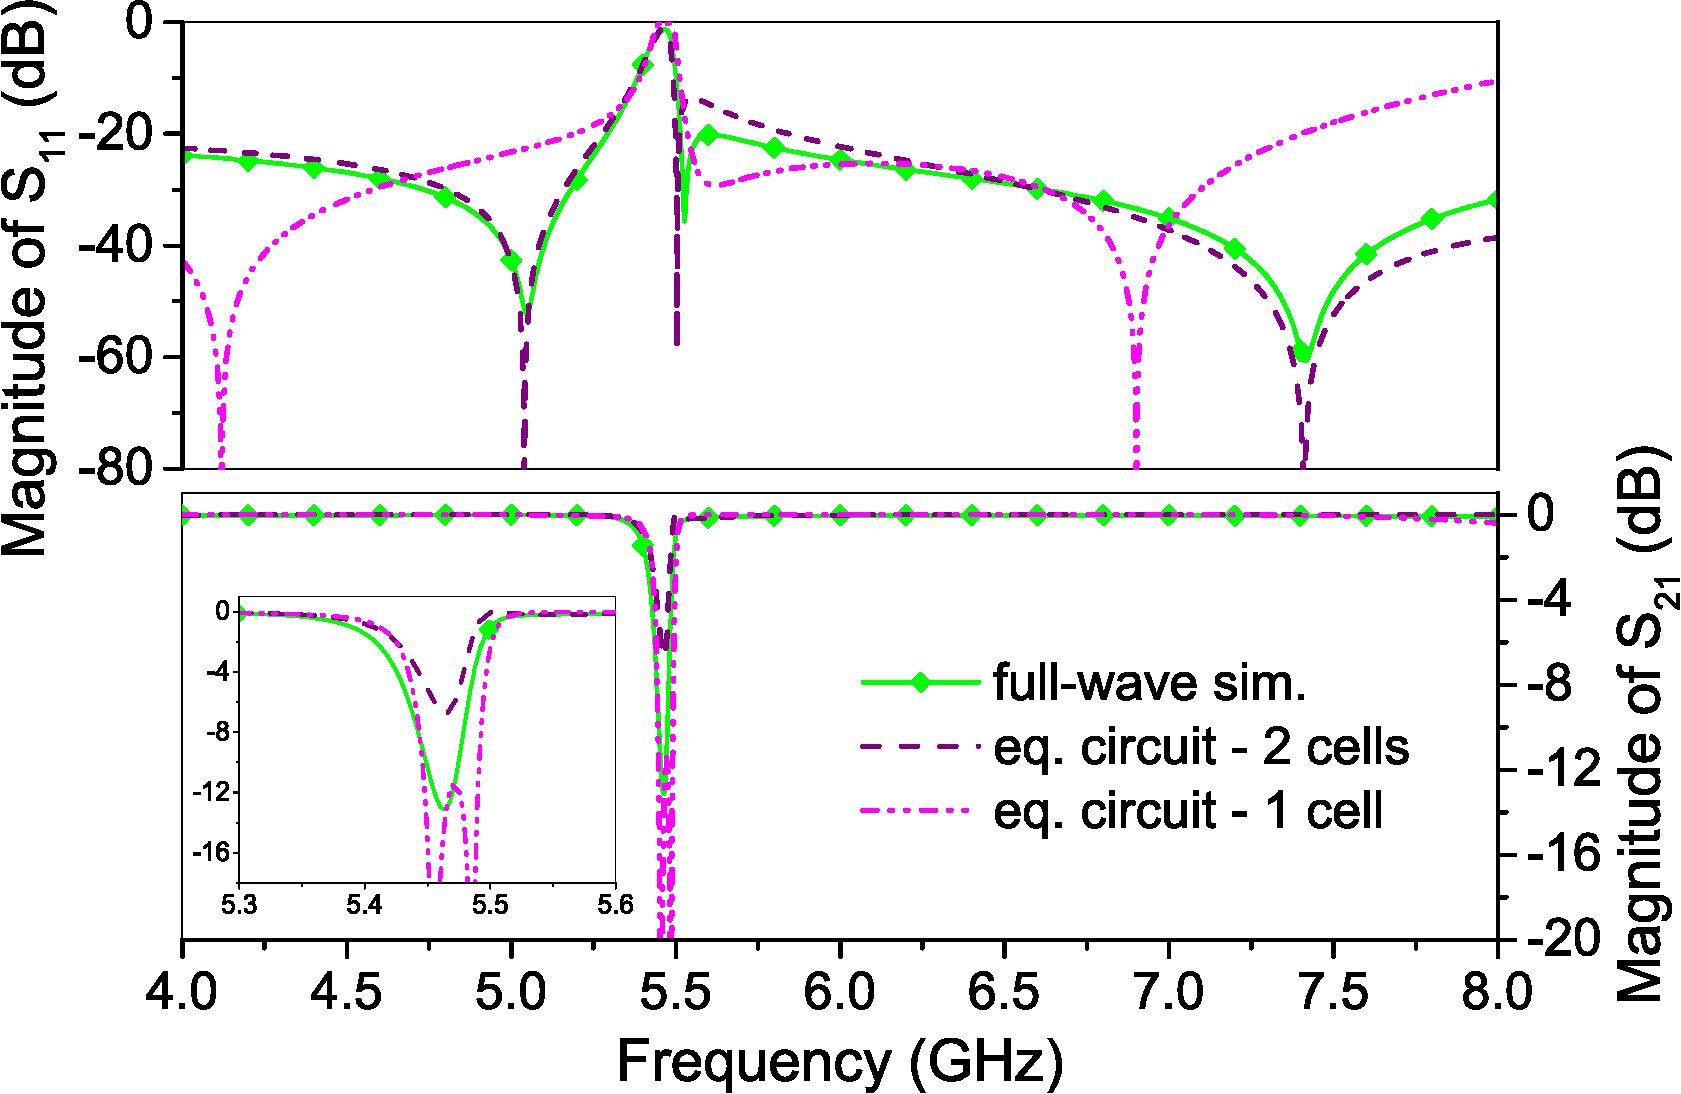
\includegraphics[width=\SirB]{sl_ekv/fig16a}
\label{f16a}}\\
\subfloat[]{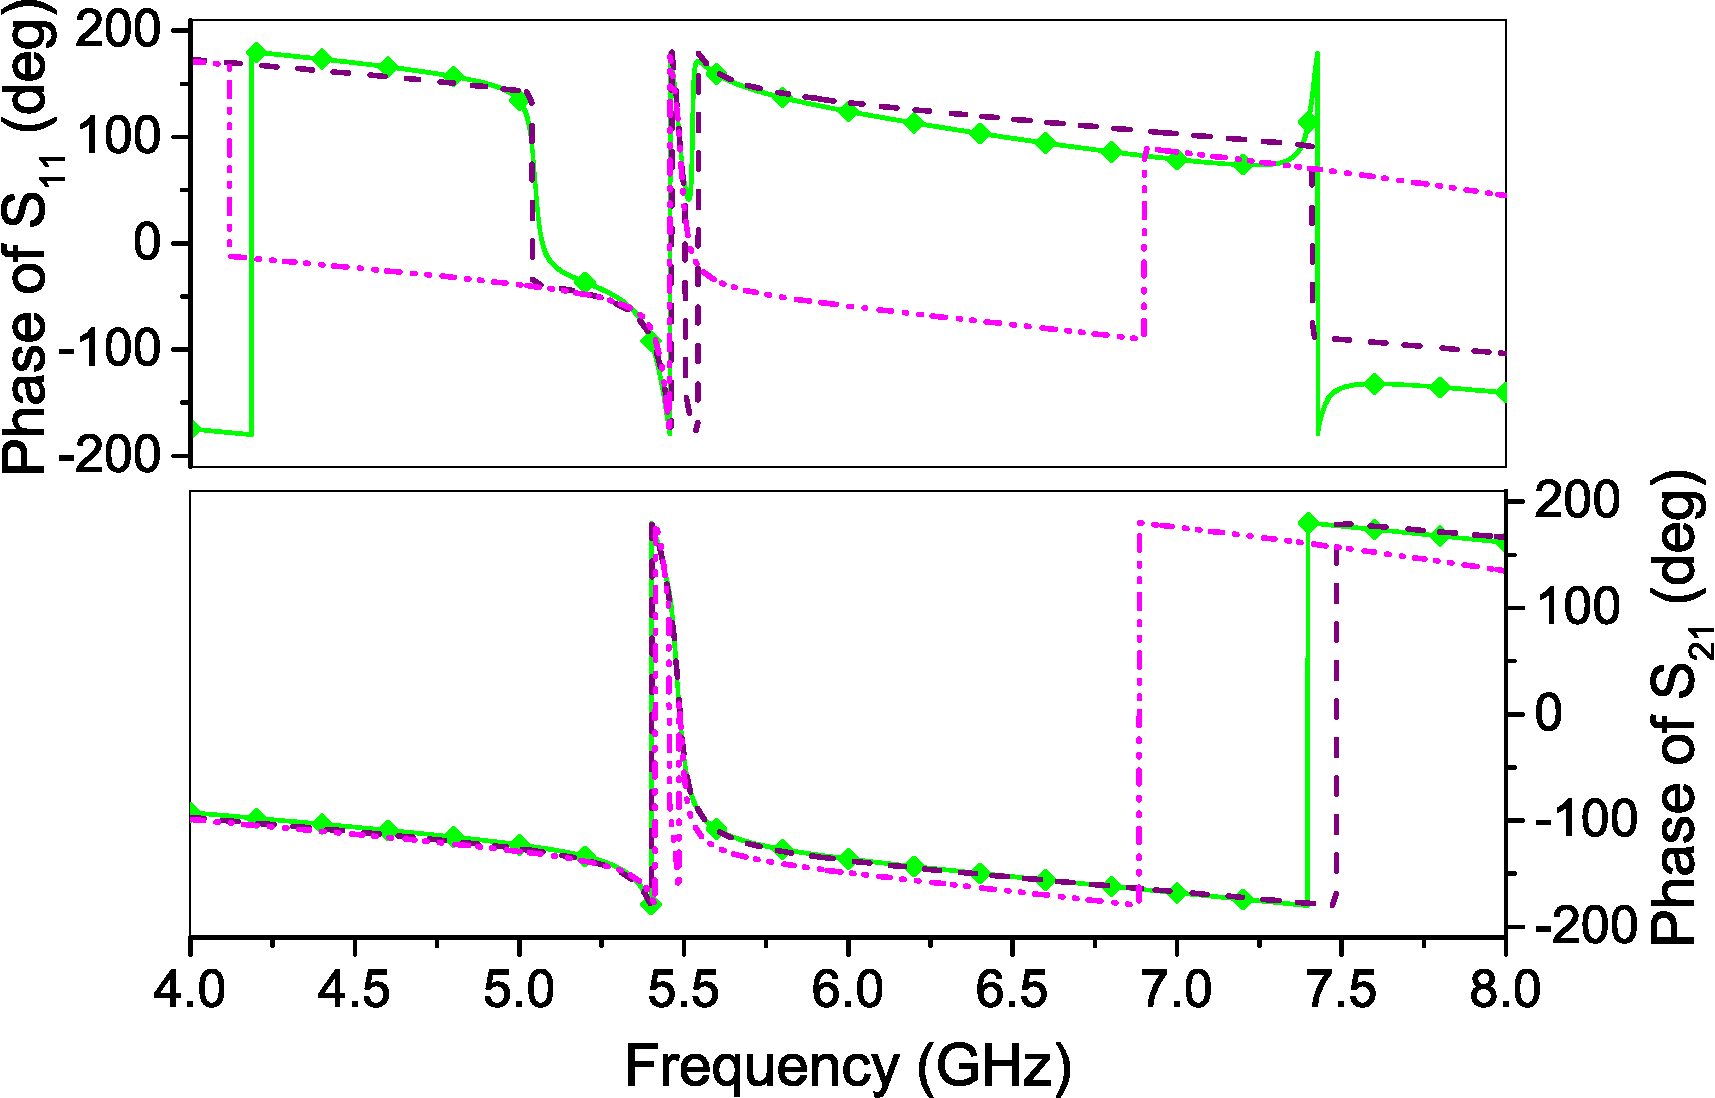
\includegraphics[width=\SirB]{sl_ekv/fig16b}
\label{f16b}}
\caption{Поређење магнитуда (а) и фаза (б) за $Ѕ$-параметре добијене мерењем, симулацијом и на основу еквивалентне шеме са једном и две П-ћелије за конфигурацију са \Fig{fk}, за растојање $D=0.5\,\mathrm{mm}$.}
\label{f16}
\end{figure}
%%%%%%%%%%%%%%%%%%%%%%%%%%%%%%%%%%%%%%%%%%%%%%%%%%%%%%%%%%%%%%%%%%%%%%%%%%
Резултати симулације и еквивалентне шеме са једном и две П-ћелије за конфигурацију са \Fig{fk}, за растојање између резонатора $D=0.5\,\mathrm{mm}$, приказани су на \Fig{f16}. Веома добро слагање добијено је у целом опсегу од интереса, и у магнитуди и у фази $Ѕ$-параметара, за модел са две П-ћелије. Насупрот томе, модел са једном П-ћелијом није у стању да поклопи рефлексију, осим у уском опсегу око резонансе. Вредности коефицијената спреге добијене су фитовањем, и износе $k_m=0.1$ и $k_{mc}=0.015$.

%%%%%%%%%%%%%%%%%%%%%%%%%%%%%%%%%%%%%%%%%%%%%%%%%%%%%%%%%%%%%%%%%%%%%%%%%%
\section{Закључак}
%%%%%%%%%%%%%%%%%%%%%%%%%%%%%%%%%%%%%%%%%%%%%%%%%%%%%%%%%%%%%%%%%%%%%%%%%%
Предложена је унапређена еквивалентна шема за микрострип вод оптерећен сплит-ринг резонаторима. Различите оријентације СРР-а у односу на вод су анализиране: са паралелним процепом ближе и даље воду, као и са нормалним процепом. Штампани вод може бити спрегнут са једним СРР-ом са једне стране, или са два СРР-а постављена симетрично/асиметрично са обе стране вода. Овакве структуре испољавају одзив филтра непропусника опсега, али се предложене еквивалентне шеме лако могу модификовати у пропуснике опсега додавањем паралелне индуктивности.

Без обзира да ли је у питању структура са једним или два симетрична СРР-а, користи се иста еквивалентна шема, само са различитим параметрима. Неки од њих се одређују на основу модела вишепроводничког вода ($L$, $C$, $L_s$) док се преостали ($C_s$ и $k_m$) добијају на основу аналитичких израза који их повезују са карактеристичним фреквенцијама -- резонансом и минимумом коефицијента рефлексије, добијеним из симулације. Једини параметар који је неопходно оптимизовати јесте електрична спрега присутна у случају СРР-а са нормалним процепом.

Најважнија предност предложеног модела са две ћелије јесте приближно двоструко већи опсег у коме је могуће преклопити минимум рефлексије добијен из симулације. Ово је постигнуто без повећања параметара кола у односу на модел са једном ћелијом. Такође, унапређена еквивалентна шема боље апроксимира дистрибуирану природу вода, и помера паразитни минимум рефлексије изнад резонансе СРР-а на значајно више фреквенције, у поређењу са моделом са једном ћелијом. Због свега тога, фреквенцијски опсег са добрим поклапањем је значајно увећан.

Више узорака је фабриковано и измерено како би се валидирала процедура екстракције параметара. Врло добро слагање између измерених и симулираних $Ѕ$-параметара и предложене унапређене шеме добијено је у широком фреквенцијском опсегу, и у магнитуди и у фази. Насупрот томе, показано је да конвенционални модел са једном ћелијом ради добро само у уском опсегу. Предложени модел се лако примењује на каскадиране структуре, као што је демонстрирано са две јединичне ћелије са различитим међусобним растојањима. Каскадирани модел је валидиран помоћу симулације, и веома добро слагање је добијено.

psgpar

\documentclass[main.tex]{subfiles}

\begin{document}

\chapter{Теорија спрегнутих модова}
\label{ch:tsm}

\section{Апстракт}
У овом поглављу биће изложене основе теорије спрегнутих модова, која представља веома погодан алат за анализу расејања у системима спрегнутих резонатора. Затим ће метода бити примењена на јединичне ћелије микроталасних метаматеријала. Апроксимативни аналитички облици параметара расејања. Поређење са еквивалентним шемама. Антисиметрични модели.

\section{Увод}
\subsection{Мотивација}%
У претходној глави приказано је моделовање јединичних ћелија микроталасних метаматеријала помоћу еквивалентних шема. Овакав начин анализе се преовлађујуће користи у литератури, и примењив је на широк спектар различитих структура и повезаних ефеката~\cite{baena,aznar_improved,naqui:13,radoman}.
%\emph{још неке реф! промени мало ову реченицу}.
Упркос томе, апроксимација помоћу еквивалентне шеме инхерентно поседује неке особине, које се могу показати као нежељене.
На пример, структура по којој се простире вођени талас (вод или таласовод) моделује се као једна или више секција елемената са концентрисаним параметрима (калема и кондензатора), што у суштини представља нископропусни филтар. Ово може узроковати нефизичке резонансе.
% можда боље да не тупим о овоме?
Конкретно, често је пожељно имати (апроксимативне) изразе за параметре расејања -- рефлексију и трансмисију. У овом раду то је мотивисано жељом за проучавањем ефекта класичне аналогије електромагнетно индуковане транспаренције (ЕИТ). У принципу, параметре расејања је увек могуће израчунати полазећи од еквивалентне шеме, међутим показује се да то није најпогоднији приступ. Разлог за то је што еквивалентна шема, у суштини, представља графички начин за репрезентацију система диференцијалних једначина за струје и напоне. За расејање се, насупрот томе, користе таласни параметри, који се могу интерпретирати као други базис за опис поља на воду.\footnote{Због краткоће, у овој глави ћемо надаље говорити само о водовима, имајући у виду било коју структуру за вођење електромагнетног таласа.} Природније је проблем разматрати у овом базису, што нам управо омогућава теорија спрегнутих модова (ТСМ).
% можда овде коментар око апроксимације вода (нископропусност, паразитне резонансе)
\subsection{Историјат}
Прва појављивања теорије спрегнутих модова у литератури потичу из 1950-их година, управо у области микроталасне технике. Била је примењена за анализу цеви са путујућим таласом~\cite{pierce1954coupling}, \foreign{backward-wave} осцилатора~\cite{1471949}, као и параметарских појачавача, осцилатора и конвертора фреквенције~\cite{louisell1960coupled}. Паралелно су се јавиле примене у таласоводима~\cite{1124830,louisell1955analysis}, где су касније укључене и периодичне структуре~\cite{tang1969mode}.

Ови први радови нису били строго формално засновани, већ су модови идентификовани на основу искуства, а њихова динамика је извођена из енергетских разматрања. Ригорозно извођење ТСМ дао је Шелкунов, помоћу развоја поља преко модова неспрегнутог система~\cite{6771476}. Једначине ТСМ су еквивалентне Максвеловим једначинама уколико модови чине комплетан скуп. У пракси, обично се користи мањи број модова; у том случају једначине ТСМ могу се извести из варијационог принципа, при чему стационарност обезбеђује могућност добре апроксимације~\cite{hausproc}.

Током седамдесетих година, ТСМ је развијена за оптичке таласоводе~\cite{6771781,snyder1972coupled,1077767}. Успешно је примењивана за анализу многих оптоелектронских и фибер оптичких уређаја, као што су различити таласоводи и оптичка влакна~\cite{taylor1973optical,mcintyre1973power}, спрежници~\cite{1069190}, ласери~\cite{butler1984coupled}, итд.
%Ипак, касније се почела више асоцирати са оптичким резонаторима у фотоници~\cite{hausproc,Fan:03}.

У класичној ТСМ претпоставка је да су модови међусобно ортогонални, што је испуњено уколико се разматра јединствена структура без губитака. Уколико се за експанзију користе модови различитих референтних структура, ортогоналност не мора нужно да важи. У том случају класична формулација ТСМ није коректна, због чега је у новије време развијана неортогонална ТСМ~\cite{haus1987coupled,wonjoo}.

% ovaj pasus nikako ne valja!!
Независна променљива у ТСМ може бити или просторна координата или време; у зависности од тога говоримо о спрезању модова у простору или времену~\cite{haus}. Просторна варијанта ТСМ коришћена је за анализу периодичних структура, нпр. микрострип водова са периодичним пертурбацијама у проводној равни, који припадају класи тзв. структура са фотонским зонским процепом (\foreign{photonic band-gap, PBG})~\cite{lopetegi_cmt}. Временска (темпорална) ТСМ није примењивана за проучавање структура на бази метаматеријала у микроталасном опсегу...

\subsection{Хеуристички приступ}

У овој секцији биће изложене основе теорије спрегнутих модова, следећи~\cite{haus}. Овај приступ није строго формалан, и донекле се заснива на интуитивним аргументима. Међусобни утицаји различитих модова ће се узимати преко линеарних чланова; математички, ово је апроксимација која је оправдана ако је спрега слаба. Касније... Претпостављаће се да су сви системи без губитака; уколико је потребно, губици се могу узети у обзир као додатна пертурбација~\cite{haus}.
% можда нешто треба рећи о теорији пертурбација (апрокс 1. реда итд.)

\begin{figure}[h]
\centering
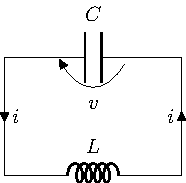
\includegraphics[width=0.4\linewidth]{sl_tsm/lckolo.pdf}
\caption{Резонантно коло.}
\label{tsm:fig:lckolo}
\end{figure}
Прво ће бити размотрено $LC$ колo као пример изолованог резонатора (сл.~\ref{tsm:fig:lckolo}). Напон и струја задовољавају диференцијалне једначине:
\begin{equation}
v = L \frac{d i}{d t}; \qquad i = -C \frac{d v}{d t}.
\end{equation}
Сменом се лако може добити једначина линеарног хармонијског осцилатора, са резонантном фреквенцијом $\omega_0 = \frac{1}{\sqrt{LC}}$. \emph{Амплитуда позитивне фреквенције} дефинише се као:
\begin{equation}
\alpha = \sqrt{\frac{C}{2}}\left( v + j\sqrt{\frac{L}{C}}i  \right),
\label{tsm:pamp}
\end{equation}
која задовољава диференцијалну једначину првог реда
\begin{equation}
\frac{d\alpha}{dt} = j\omega_0 \alpha.
\label{tsm:smdif1}
\end{equation}
Нормализација у \ref{tsm:pamp} је погодно одабрана тако да квадрат амплитуде $\alpha$ одговара снази:
\begin{equation}
|\alpha|^2 = \frac{C}{2}|V|^2 = W,
\end{equation}
док фаза одговара тренутној фази осцилација. За комплетан опис, потребно би било увести и променљиву, комплексно-конјуговану у односу на (\ref{tsm:pamp}), али показује се да је њу могуће занемарити. На овај начин је опис резонатора поједностављен.

\begin{figure}[h] 
\centering
\includegraphics[width=0.4\linewidth]{sl_tsm/sm-vod1.pdf}
\caption{Спрега резонантног мода и вода.}
\label{tsm:fig:slike/smfig}
\end{figure}
Наравно, случај усамљеног резонатора није посебно занимљив; права вредност овог приступа се показује приликом разматрања спреге са водом. На сл.~ приказан је најједноставнији случај. У овом случају, јављају се два ефекта:
\begin{itemize}
\item енергија резонатора ,,цури`` у таласе на воду, што резонантни мод види као ефективне губитке;
\item инцидентни таласи врше побуду резонантног мода.
\end{itemize}
Најједноставнији пример шематски је приказан на сл.~\ref{tsm:fig:slike/smfig}, где је вод на свом крају спрегнут са резонантним модом. Поље на воду описано је таласним коефицијентима инцидентног, $a$, и рефлектованог таласа, $b$, према уобичајеној дефиницији за $S$-параметре. Математички, једначина (\ref{tsm:smdif1}) ће бити модификована на следећи начин
\begin{equation}
\frac{d\alpha}{dt} = j\omega_0 \alpha - \gamma \alpha + \kappa a,
\label{tsm:smdif2}
\end{equation}
где $\gamma$ представља коефицијент слабљења, а $\kappa$ коефицијент спреге инцидентног таласа и резонантног мода. За побуду константне фреквенције $\omega$, решење (\ref{tsm:smdif2}) гласи:
\begin{equation}
\alpha = \frac{\kappa a}{j(\omega-\omega_0) + \gamma}.
\label{tsm:haus:pobuda}
\end{equation}
С друге стране, рефлектовани талас на воду износиће
\begin{equation}
b = S_{11}^{(0)} a + d\alpha,
\label{tsm:haus:refl}
\end{equation}
где је $S_{11}^{(0)}$ коефицијент рефлексије у одсуству резонатора, а $d$ коефицијент спреге са рефлектованим таласом. Полазећи од закона одржања енергије, и симетрије Максвелових једначина у односу на измену знака времена, показује се да важи
\begin{equation}
\kappa = d,\qquad \gamma = \frac{1}{2}|d|^2.
\end{equation}
Комбиновањем (\ref{tsm:haus:pobuda}) и (\ref{tsm:haus:refl}) лако се добија израз за модификовани коефицијент рефлексије услед присуства резонатора:
\begin{equation}
S_{11} = \frac{b}{a} = S_{11}^{(0)} + \frac{d}{j(\omega-\omega_0) + {|d|^2}/{2}}.
\end{equation}

У случају два међусобно спрегнута резонатора, динамика система има следећи облик:
\begin{eqnarray}
\frac{d\alpha_1}{dt} & = j\omega_1 \alpha_1 + \kappa_{12} \alpha_2 , \\
\frac{d\alpha_2}{dt} & = j\omega_2 \alpha_2 + \kappa_{21} \alpha_1 , 
\label{tsm:haus:2sprenuta}
\end{eqnarray}
при чему због одржања енергије важи $\kappa_{12} = \kappa_{21}$.

Изразе (\ref{tsm:smdif1})--(\ref{tsm:haus:2sprenuta}) могуће је генералисати на случај $n$ (потенцијално спрегнутих) резонатора и $m$ улазно/излазних таласних портова
\begin{align}
\frac{\partial}{\partial t}
\begin{bmatrix}
\alpha_1 \\ \vdots \\ \alpha_n
\end{bmatrix}
& = \left(j\mathbf{\Omega} - \mathbf{\Gamma} \right)\begin{bmatrix}
\alpha_1 \\ \vdots \\ \alpha_n
\end{bmatrix}
+ \mathbf{D}^T
\begin{bmatrix}
a_1 \\ \cdots \\ a_m
\end{bmatrix}
\label{tsm:haus:evomat}\\
\intertext{за резонаторе, и}
\begin{bmatrix}
b_1 \\ \vdots \\ b_m
\end{bmatrix}
& = \mathbf{S}^{(0)}
\begin{bmatrix}
a_1 \\ \vdots \\ a_m
\end{bmatrix}
+\mathbf{D}\begin{bmatrix}
\alpha_1 \\ \vdots \\ \alpha_n
\end{bmatrix};
\label{tsm:haus:reflmat}
\end{align}
за рефлектоване таласе, где су
\begin{equation}
\mathbf{\Omega} = \begin{bmatrix}
\omega_1      & \cdots    & \kappa_{1n} \\
\vdots        & \ddots    & \vdots      \\
\kappa_{1n}^* & \cdots    & \omega_n    \\
\end{bmatrix}; \qquad
\mathbf{D} = \begin{bmatrix}
d_{11}  & \cdots  & d_{1m} \\
\vdots  & \ddots  & \vdots \\
d_{n1}  & \cdots  & d_{nm} \\
\end{bmatrix};\qquad \mathbf{\Gamma}=\frac{1}{2}\mathbf{D}^\dag \mathbf{D};
\label{tsm:haus:wdmat}
\end{equation}
а $\mathbf{S}^{(0)}$ представља ,,директну`` матрицу расејања, која карактерише систем у одсуству резонатора. Додатно, може се показати да важи следећа релација
\begin{equation}
\mathbf{S}^{(0)}\mathbf{D^*}=-\mathbf{D},
\label{tsm:haus:d_usl}
\end{equation}
помоћу које је могуће одредити фазе елемената матрице $\mathbf{D}$~\cite{wonjoo}.

%Изрази (\ref{tsm:cm_s21})--(\ref{tsm:cm_s11}) представљају рационалне функције. However, compared to the general methods~\cite{rationalfit}, CMT enables exploiting system geometry and significantly reducing the number of unknown parameters. Also, if field patterns of modes are known, CMT constants can be directly calculated~\cite{hausproc}.

\section{Примена? Резултати?}
\subsection{Антисиметрични сплит рингови}%

Микрострип водови, оптерећени са СРР резонаторима са варијабилним положајем процепа, приказани су на сл.~\ref{tsm:sl1a}-\ref{tsm:sl1}. У општем случају, постојаће спрега између два СРР-а, на основу чега се очекују две резонансе у спектру, услед цепања(?). Геометрије на сл.~\ref{tsm:sl1a} поседују рефлексиону симетрију у односу на раван, нормалну на супстрат, која садржи централну осу вода. Због ове симетрије, један мод не може бити побуђен, због чега ће бити присутна само једна резонанса у трансмисији~\cite{radoman}. С друге стране, геометрије на сл.~\ref{tsm:sl1}, које ћемо називати \emph{антисиметричним}, не поседују раван симетрије; уместо тога, симетричне су у односу на ротацију од \SI{180}{\degree} око централне тачке. У наставку ће ТСМ и анализа помоћу еквивалентне шеме бити примењена на структуре са сл.~\ref{tsm:sl1}.

Оно што антисиметричне структуре чини занимљивим јесте да испољавају мешовиту (електричну и магнетну) спрегу СРР-ова са водом, као и незанемарљиву спрегу између самих прстенова, а притом су електрично симетричне, због чега је могуће поједностављено их анализирати преко парне и непарне побуде. За разлику од структура са раванском симетријом, поседују две резонансе у трансмисионом спектру, које се могу независно подешавати. Са практичне тачке гледишта, ове структуре могу послужити као основа занимљивих ефеката, као што је класична аналогија ЕИТ-а~\cite{tassin:09,mr03:eit,cihan}. %These properties are suitable for various applications like slow light, delay lines and sensors.

\begin{figure}[!t]
\centering
\subfloat[]{\includegraphics[width=0.42\columnwidth]{sl_tsm/pod0_1.jpeg}
\label{tsm:sl1:sim1}}%
\hfil
\subfloat[]{\includegraphics[width=0.42\columnwidth]{sl_tsm/pod90sim.jpeg}
\label{tsm:sl1:sim2}}\\
\subfloat[]{\includegraphics[width=0.42\columnwidth]{sl_tsm/pod90sim_cosak.jpeg}\label{tsm:sl1:sim3}}%
\hfil
\subfloat[]{\includegraphics[width=0.42\columnwidth]{sl_tsm/pod180x2.jpeg}}
\caption{Микрострип вод спрегнут са два СРР-а у симетричној конфигурацији.}
\label{tsm:sl1a}
\end{figure}
\begin{figure}[!t]
\centering
\subfloat[]{\includegraphics[width=0.48\columnwidth]{sl_tsm/pod0.jpeg}\label{tsm:sl1:pod0}}
\hfil
\subfloat[]{\includegraphics[width=0.48\columnwidth]{sl_tsm/pod180.jpeg}
\label{tsm:sl1:pod180}}\\
\subfloat[]{\includegraphics[width=0.48\columnwidth]{sl_tsm/pod90bg.jpeg}
\label{tsm:sl1:pod90bg}}%
\hfil
\subfloat[]{\includegraphics[width=0.42\columnwidth]{sl_tsm/pod90dv.jpeg}
\label{tsm:sl1:pod90dv}}\\
\subfloat[]{\includegraphics[width=0.48\columnwidth]{sl_tsm/pod90sr.jpeg}\label{tsm:sl1:pod90sr}}%
\caption{Микрострип вод спрегнут са два СРР-а у антисиметричној конфигурацији.}
\label{tsm:sl1}
\end{figure}

\subsection{Анализа помоћу ТСМ}\label{tsm:sec:cmt}
\begin{figure}
\centering
\includegraphics[scale=1]{sl_tsm/smfig.pdf}
\caption{Вод бочно спрегнут са два резонатора.}
\label{tsm:smfig}
\end{figure}

Шематски приказ геометрија са сл.~\ref{tsm:sl1a}--\ref{tsm:sl1}, у контексту ТСМ, дат је на сл.~\ref{tsm:smfig}. Систем се састоји од два резонатора и поседује два улазно/излазна порта, због чега димензије матрица $\mathbf{D}$, $\mathbf{S}$ и $\mathbf{\Omega}$, дефинисаних у (\ref{tsm:haus:wdmat}), износе $2\times 2$. Узимајући у обзир ротациону симетрију система, може се закључити да ове матрице имају следећи облик:
\begin{equation}
\mathbf{S}^{(0)} = \begin{bmatrix}
S^{(0)}_{11} & S^{(0)}_{21} \\
S^{(0)}_{21} & S^{(0)}_{11}
\end{bmatrix},\qquad
\mathbf{D} = \begin{bmatrix}
d_1 & d_2 \\
d_2 & d_1
\end{bmatrix},\qquad
\mathbf{\Omega} = \begin{bmatrix}
\omega_0 & -\kappa \\
-\kappa & \omega_0
\end{bmatrix},
\label{tsm:haus:sims}\end{equation}
при чему $\kappa\in \mathbb{R}$ у овом случају. У устаљеном режиму побуде, после замене (\ref{tsm:haus:evomat}) и (\ref{tsm:haus:sims}) у (\ref{tsm:haus:reflmat}), лако се добија решење за укупну трансмисију кроз систем:
\begin{equation}
\begin{split}
S_{21} = S^{(0)}_{21} + \frac{(d_1+d_2)^2}{2j(\omega-\omega_0 - \kappa) + |d_1+d_2|^2}\\
- \frac{(d_1-d_2)^2}{2j(\omega-\omega_0 + \kappa) + |d_1-d_2|^2},
\end{split}\label{tsm:cm_s21}
\end{equation}
и за рефлексију:
\begin{equation}
\begin{split}
S_{11} = S^{(0)}_{11} + \frac{(d_1+d_2)^2}{2j(\omega-\omega_0 - \kappa) + |d_1+d_2|^2}\\
+ \frac{(d_1-d_2)^2}{2j(\omega-\omega_0 + \kappa) + |d_1-d_2|^2}.
\end{split}\label{tsm:cm_s11}
\end{equation}
У изразима (\ref{tsm:cm_s21})-(\ref{tsm:cm_s11}), први разломак одговара парном (симетричном) а други немарном (антисиметричном) моду спрегнутих резонатора. Резонантне учестаности ових модова су $\omega_{\pm} = \omega_0 \pm \kappa$ и $Q$-фактори:
\begin{equation}
Q_\pm = \nicefrac{\omega_\pm}{\gamma_{\pm}},\qquad \gamma_{\pm} = |d_1 \pm d_2|^2
\end{equation}
где знак (+) одговара парном, а (-) непарном моду.
% * <vojislav_m@yahoo.com> 2017-11-01T16:59:28.761Z:
% 
% > where (+) sign corresponds to the even mode, and (-) to the odd mode.
% proveriiii!!!!
% 
% ^.

\subsection{Анализа помоћу еквивалентне шеме}\label{tsm:sec:eqcirc}
Еквивалентна шема за антисиметричну геометрију (сл.~\ref{tsm:sl1}) приказана је на сл.~\ref{tsm:sl3}. Укључује електричну и магнетну спрегу СРР-ова са водом, као и међусобну спрегу СРР-ова. Због једноставности, за анализу у овој секцији биће коришћена шена са једном П-ћелијом; приликом поређења резултата биће укључена и шема са две ћелије.

Шема са сл.~\ref{tsm:sl3} је електрично симетрична, због чега је погодно анализирати је преко парне/непарне побуде~\cite{hong}. Међутим, она не поседује рефлексиону симетрију, због чега није могуће одредити парне и непарне адмитансе на стандардни начин, постављањем електричног и магнетног зида у равни симетрије. Уместо тога, биће показано како се ротациона симетрија кола може искористити да се добију тражене адмитансе.

На почетку приметимо да сви одзиви у колу представљају билинеарне функције улазних параметара, нпр.
\begin{equation}
I_{S1} = \mathcal{L}_{I_{S1}}(V_1,V_2) = -\mathcal{L}_{I_{S1}}(-V_1,-V_2).
\label{tsm:blin1}\end{equation}
Услед антисиметрије, следећа релација мора важити (за референтне смерове са сл.~\ref{tsm:sl3}):
\begin{equation}
    I_{S2}=\mathcal{L}_{I_{S2}}(V_1,V_2)=\mathcal{L}_{I_{S1}}(V_2,V_1).
\label{tsm:blin2}\end{equation}
\begin{table}[!t]
\renewcommand{\arraystretch}{1.3}
\caption{Одзиви у еквивалентном колу за парну и непарну побуду.}
\label{tsm:tabela_uslovi}
\centering
\begin{tabular}{|c|c|}
\hline
парна & непарна \\
\hline
$V_1 = V_2$ & $V_1 = -V_2$ \\
\hline
$I_{S1} = I_{S2}$ & $I_{S1} = -I_{S2}$ \\
\hline
$V_{S1} = V_{S2}$ & $V_{S1} = -V_{S2}$ \\
\hline
$I_L = 0$ & $I_L$ произвољно\\
\hline
\end{tabular}
\end{table}
\begin{figure}
    \begin{center}
        \includegraphics[scale=1]{sl_tsm/sl3.pdf}
    \caption{Еквивалентна шема за структуре са сл.~\ref{tsm:sl1}.}
    \label{tsm:sl3}
  \end{center}
\end{figure}
\begin{figure}[!t]
\centering
\subfloat[]{
\includegraphics[scale=1.3]{sl_tsm/ekv_par.pdf}\label{tsm:ekv_par}}
\hfil
\subfloat[]{
\includegraphics[scale=1.3]{sl_tsm/ekv_nepar.pdf}\label{tsm:ekv_nepar}}
\caption{Еквивалентна шема за (а) парну и (б) непарну побуду ($L_k=k_{m12}L_S$).}
\label{tsm:sl4}
\end{figure}
Коришћењем (\ref{tsm:blin1}) и (\ref{tsm:blin2}), могуће је одредити релације за одзиве у колу, при парној и непарној побуди, и оне су сумиране у табели~\ref{tsm:tabela_uslovi}. На основу тога, могуће је одредити поједностављена кола за парну и непарну екситацију, која су приказана на сл.~\ref{tsm:sl4}. На основу њих можемо израчунати парну и непарну адмитансу, $y_{e,o}$, нормализовану на $Y_0=\sqrt{C/L}$
%\begin{equation}
%\begin{aligned}
%Y_e &=j\omega\frac{C}{2}\left(1-2k_e^2+\chi\right); \\
%Y_o &=j\omega\frac{C}{2}\left(1-2k_e^2\right) - \frac{2j}{\omega L}\xi;\\
%\chi &=\frac{2k_e^2}{1-\omega ^2 C_S L_S(1-k_{m12})}; \\
%\xi &= \frac{1 - \omega ^2 \left( C_S L_S(1+k_{m12})-2C_m L_m+k_e^2 \frac{LC}{2}\right)}{1-\omega^2C_S L_S \left(1+k_{m12}-2k_m^2\right)}.
%\end{aligned}
%\end{equation}
\begin{equation}
\begin{aligned}
y_e &= y_e^\Pi + \frac{j}{2}\frac{\omega}{\omega_{LC}}\frac{2\gamma_e^2}{1-\omega^2 / \omega_e^2}, \\
y_e^\Pi &= \frac{j}{2}\frac{\omega}{\omega_{LC}}\left(1 - 2 k_e^2\right), \\
y_o &=  y_o^\Pi + \frac{j}{2}\frac{\omega}{\omega_{LC}}\frac{2\gamma_o^2}{1-\omega^2 / \omega_o^2}, \\
y_o^\Pi &= \frac{j}{2}\frac{\omega}{\omega_{LC}}\left(1 - 2 k_e^2\right) - 2j\frac{\omega_{LC}}{\omega}
;
\end{aligned}
\label{tsm:eo}
\end{equation}
где је
\begin{equation}
\begin{aligned}
\gamma_e &= k_e, \\
\gamma_o &= 2\omega_{LC}\sqrt{L_S C_S} k_m - k_e, \\
\omega_e &= 1/ \sqrt{L_S C_S(1-k_{m12})}, \\
\omega_o &= 1/ \sqrt{L_S C_S(1+k_{m12}-2k_m^2)}, \\
\omega_{LC} &= 1/ \sqrt{LC}.
\end{aligned}
\label{tsm:eo_pom}
\end{equation}
У (\ref{tsm:eo}) раздвојени су нерезонантни делови адмитанси преко чланова $y_{e,o}^\Pi$. Они представљају парну  и непарну адмитансу само П-ћелије на.~\ref{tsm:sl3}, односно потичу само од вода.\footnote{Треба приметити да су $y_{e,o}^\Pi$ пертурбовани у односу на изоловани вод, услед присуства СРР-ова, али овај ефекат је врло мали.} Ова нотација ће олакшати поређење са резултатима ТСМ, као што ће се видети касније. Према~\cite{hong}, коефицијент трансмисије, $S_{21}$, износи:
\begin{equation}
\begin{aligned}
S_{21} =& \frac{1}{2}(S_{11,e}-S_{11,o}) \\
=& \frac{1}{2}\left( \frac{1-y_e}{1+y_e}
- \frac{1-y_o}{1+y_o} \right).
\end{aligned}
\end{equation}
Нерезонантни део трансмисије може се изразити преко чланова $y_{e,o}^\Pi$ (\ref{tsm:eo}):
\begin{equation}
S_{21}^\Pi = \frac{1}{2} \left( S_{11e}^\Pi - S_{11o}^\Pi \right),\quad
S_{11e,o}^\Pi = \frac{1-y_{e,o}^\Pi}{1+y_{e,o}^\Pi},
\label{tsm:spi}\end{equation}
Што је еквивалентно матрици ,,директног`` расејања $\mathbf{S}^{(0)}$ из секције~\ref{tsm:sec:cmt}. Заменом (\ref{tsm:eo}), (\ref{tsm:eo_pom}) и (\ref{tsm:spi}), после сређивања, добија се коначни израз за трансмисију:
\begin{equation}
S_{21} = S_{21}^\Pi - \frac{S_{11,e}^\Pi\gamma'_e}{j(\omega^2-\varpi_e^2)+\gamma'_e} + \frac{S_{11,o}^\Pi\gamma'_o}{j(\omega^2-\varpi_o^2)+\gamma'_o},
\label{tsm:s21sm}\end{equation}
где је
\begin{equation}
\gamma'_{e,o} = \operatorname{Re}\left\{ \frac{1}{1+y_{e,o}^\Pi} \right\} \frac{\omega}{\omega_{LC}}\omega_{e,o}^2\gamma_{e,o}^2,
\label{tsm:gama}\end{equation}
\begin{equation}
\varpi_{e,o} = \omega_{e,o} - \operatorname{Im}\left\{ \frac{1}{1+y_{e,o}^\Pi} \right\} \frac{\omega}{\omega_{LC}}\omega_{e,o}^2\gamma_{e,o}^2.
\label{tsm:omega}\end{equation}
Облик (\ref{tsm:s21sm}) је намерно изабран како би се нагласила аналогија са резултатом ТСМ (\ref{tsm:cm_s21}). Важна разлика је да, уместо константних вредности за ТСМ, у (\ref{tsm:s21sm}) имамо функције учестаности, дефинисане са (\ref{tsm:gama})-(\ref{tsm:omega}). Ипак, ове функције споро варирају у поређењу са резонантним члановима, због чега су оба израза приближно еквивалентна у околини резонанси. У табели~\ref{tsm:tabela_ekv} приказано су релације које повезују параметре кола са константама за ТСМ, које се могу одредити на овај начин фиксирањем $\omega$ на жељеној фреквенцији.
\begin{table}[!t]
\renewcommand{\arraystretch}{2.8}
\caption{Релације између константи за ТСМ и параметара кола.}
\label{tsm:tabela_ekv}
\centering
\begin{tabular}{|c|c|}
\hline
ТСМ & Еквивалентна шема \\
\hline
$\omega_+$ & $\omega_{e} - \operatorname{Im}\left\{ \frac{1}{1+y_{e}^\Pi} \right\} \frac{\omega\omega_{e}^2}{\omega_{LC}(\omega + \omega_e)}\gamma_{e}^2$ \\
\hline
$\omega_-$ & $\omega_{o} - \operatorname{Im}\left\{ \frac{1}{1+y_{o}^\Pi} \right\} \frac{\omega\omega_{o}^2}{\omega_{LC}(\omega + \omega_o)}\gamma_{o}^2$ \\
\hline
$\gamma_+$ & $\operatorname{Re}\left\{ \frac{1}{1+y_{e}^\Pi} \right\} \frac{2\omega\omega_{e}^2}{\omega_{LC}(\omega + \omega_e)}\gamma_{e}^2$ \\
\hline
$\gamma_-$ & $\operatorname{Re}\left\{ \frac{1}{1+y_{o}^\Pi} \right\} \frac{2\omega\omega_{o}^2}{\omega_{LC}(\omega + \omega_o)}\gamma_{o}^2$\\
\hline
\end{tabular}
\end{table}

Фреквенцијска зависност ефективних резонантних фреквенција модова $\varpi_{e,o}$ и јачина спреге $\gamma'_{e,o}$ у (\ref{tsm:s21sm})--(\ref{tsm:omega}) може бити образложена на следећи начин. П-ћелија која у колу представља вод се такође понаша као резонатор, додуше са знатно вишом резонантном фреквенцијом од СРР-ова. Ипак, спрега са водом узрокује фреквенцијски зависну пертурбацију, евидентну у (\ref{tsm:gama})--(\ref{tsm:omega}). Како би се добили аналитички изрази за параметре расејања, који су довољно једноставни да би били практично употребљиви, обично је неопходно занемарити овакве пертурбације. Међутим, ово није лак задатак полазећи од Кирхофових закона за еквивалентно коло, пошто је тешко унапред знати шта се може занемарити, а шта не. Насупрот томе, ТСМ даје изразе као што су (\ref{tsm:cm_s21}) директно, зато што инхерентно раздваја трансмисиони медијум и резонаторе, осим спреге првог реда. Због тога, она представља природни алат за анализу расејања у системима спрегнутих резонатора.

\section{Резултати и поређење}\label{tsm:sec:res}
\subsection{Валидација аналогије између два модела}
\begin{figure}[!t]
\centering
\includegraphics[width=7cm]{sl_tsm/dim3.jpeg}
\caption{Релевантне димензије:  $h = \SI{1.27}{\mm}$, $L_r = \SI{3}{\mm}$, $L_m = \SI{0.25}{\mm}$, $L_g = \SI{0.5}{\mm}$, $W_r = \SI{0.2}{\mm}$, $W_l = \SI{1.2}{\mm}$ и $s = \SI{0.1}{\mm}$.}
\label{tsm:dim}
\end{figure}
\begin{figure}
    \begin{center}
        \subfloat[]{\includegraphics[scale=0.7]{sl_tsm/vod1cel.pdf}\label{tsm:slvod:1cel}}\hfil
        \subfloat[]{\includegraphics[scale=0.7]{sl_tsm/vod2cel.pdf}\label{tsm:slvod:2cel}}	
    \caption{Еквивалентна шема вода са: (а) једном, и (б) две П-ћелије.}
    \label{tsm:sl:vod2cel}
  \end{center}
\end{figure}
\begin{figure}[!t]
\centering
\subfloat[]{\includegraphics[width=0.5\textwidth]{sl_tsm/pod0/c2_mag.pdf}}\\
\subfloat[]{\includegraphics[width=0.5\textwidth]{sl_tsm/pod0/c2_faza.pdf}}
\caption{Магнитуда и фаза $S$-параметара за модел са сл.~\ref{tsm:sl1:pod0}}
\label{tsm:rez1c:pod0}
\end{figure}
\begin{figure}[!t]
\centering
\subfloat[]{\includegraphics[width=0.5\textwidth]{sl_tsm/pod180/c2_mag.pdf}}\\
\subfloat[]{\includegraphics[width=0.5\textwidth]{sl_tsm/pod180/c2_faza.pdf}}
\caption{Магнитуда и фаза $S$-параметара за модел са сл.~\ref{tsm:sl1:pod180}}
\label{tsm:rez1c:pod180}
\end{figure}
Како би се тестирали предложени модели и упоредили њихови резултати, извршена је 3Д електромагнетна симулација структура са сл.~\ref{tsm:sl1}, док су \subref{tsm:sl1:pod0}, \subref{tsm:sl1:pod180}, \subref{tsm:sl1:pod90bg} и \subref{tsm:sl1:pod90sr} такође фабриковани и измерени. Релевантне димензије дате су на сл.~\ref{tsm:dim}, а коришћени диелектрични супстрат је Rogers RO3010 са $\varepsilon_r = \num{10.2}$. 

Најпре су одређени параметри еквивалентног кола. Како би се добили $L$, $C$ и $L_S$, микрострип вод и две најближе гране СРР-а су моделовани као секција вишепроводничког вода. Програм LINPAR~\cite{djordjevic1999linpar} је коришћен за нумерички прорачун квази-статичких параметара. На овај начин се добијају подужне капацитивности и индуктивности, из којих се тражене вредности $L$, $C$ и $L_S$ добијају множењем са одговарајућим дужинама~\cite{radoman}. Преостали параметри се добијају фитовањем кривих на резултате симулација.

Нелдер--Мидова симплекс метода~\cite{simplex} је коришћена за фитовање, са функцијом грешке која интеграли апсолутну разлику ($L^1$ норму) између симулираних података и параметризованог модела, у спектру од \SI{4}{\giga\hertz} до \SI{8}{\giga\hertz}:
\begin{equation}
\mathrm{Err}=\int_{f_\mathrm{min}}^{f_\mathrm{max}}\sum_{i=1}^2\sum_{j=1}^2\ \left | S_{ij}^\mathrm{model} - S_{ij}^{\mathrm{sim}} \right | df.
\end{equation}
У неким случајевима, тежинска функција је ручно повећавана у околини резонанси, како би више одговарала ускопојасној природи апроксимације. Иста процедура је коришћена у свим осталим случајевима фитовања у овој глави.

%the first question is how to generate non-resonant parameters $\mathbf{S}^{(0)}$ required in expressions (\ref{tsm:cm_s21})-(\ref{tsm:cm_s11}). Simplest approach would be to take them as constants; however, in order to make the best possible comparison with equivalent circuit analysis, we decided to use network of two $\Pi$ cells representing the transmission line (Fig.~\ref{tsm:sl:vod2cel}). In this approach, both models have essentially the same non-resonant parts, and the difference comes from the way resonators are included.
Константе за ТСМ добијене су коришћењем израза на десној страни табеле~\ref{tsm:tabela_ekv}, који су израчунати на фреквенцији између резонанси. Преостаје да се одреди матрица директног расејања $\mathbf{S}^{(0)}$, што се може извести на више начина. На пример, могле би се користити константе које би се фитовале, или би се ова матрица могла добити на основу симулације секције изолованог вода. У овом случају, $\mathbf{S}^{(0)}$ је прорачуната на основу електричне шеме кола које се састоји само од једне П-ћелије (сл.~\ref{tsm:slvod:1cel}), са истим вредностима $L$ и $C$ као у еквивалентном колу. Ово омогућава најприближније поређење два модела.

Резултати за две структуре са.~\ref{tsm:sl1} су приказани на сл.~\ref{tsm:rez1c:pod0}-\ref{tsm:rez1c:pod180}. Може се видети да се еквивалентна шема и ТСМ скоро у потпуности поклапају око резонанси, док постоје одступања у ширем опсегу, у складу са закључцима из секције~\ref{tsm:sec:eqcirc}. Надаље, оба метода показују добро поклапање са симулацијама у магнитуди и фази трансмисије ($S_{21}$ параметар) у целом опсегу; с друге стране, у случају рефлексије ($S_{11}$ параметар), добро поклапање постоји само у околини резонанси.

\subsection{Побољшани резултати}
\begin{figure}
    \begin{center}
        \includegraphics[scale=1]{sl_tsm/ekv2cel.pdf}
    \caption{Еквивалентна шема за антисиметричне структуре са две П-ћелије.}
    \label{tsm:sl:ekv2cel}
  \end{center}
\end{figure}
\begin{figure}[!t]
\centering
\subfloat[]{\includegraphics[width=0.5\textwidth]{sl_tsm/pod0/c_mag.pdf}}\\
\subfloat[]{\includegraphics[width=0.5\textwidth]{sl_tsm/pod0/c_faza.pdf}}
\caption{Магнитуда и фаза $S$-параметара за модел са сл.~\ref{tsm:sl1:pod0}}
\label{tsm:rez:pod0}
\end{figure}
\begin{figure}[!t]
\centering
\subfloat[]{\includegraphics[width=0.5\textwidth]{sl_tsm/pod180/c_mag.pdf}}\\
\subfloat[]{\includegraphics[width=0.5\textwidth]{sl_tsm/pod180/c_faza.pdf}}
\caption{Магнитуда и фаза $S$-параметара за модел са сл.~\ref{tsm:sl1:pod180}}
\label{tsm:rez:pod180}
\end{figure}
\begin{figure}[!t]
\centering
\subfloat[]{\includegraphics[width=0.5\textwidth]{sl_tsm/pod90bg/c_mag.pdf}}\\
\subfloat[]{\includegraphics[width=0.5\textwidth]{sl_tsm/pod90bg/c_faza.pdf}}
\caption{Магнитуда и фаза $S$-параметара за модел са сл.~\ref{tsm:sl1:pod90bg}}
\label{tsm:rez:pod90bg}
\end{figure}
\begin{figure}[!t]
\centering
\subfloat[]{\includegraphics[width=0.5\textwidth]{sl_tsm/pod90dv/c_mag.pdf}}\\
\subfloat[]{\includegraphics[width=0.5\textwidth]{sl_tsm/pod90dv/c_faza.pdf}}
\caption{Магнитуда и фаза $S$-параметара за модел са сл.~\ref{tsm:sl1:pod90dv}}
\label{tsm:rez:pod90dv}
\end{figure}
\begin{figure}[!t]
\centering
\subfloat[]{\includegraphics[width=0.5\textwidth]{sl_tsm/pod90sr/c_mag.pdf}}\\
\subfloat[]{\includegraphics[width=0.5\textwidth]{sl_tsm/pod90sr/c_faza.pdf}}
\caption{Магнитуда и фаза $S$-параметара за модел са сл.~\ref{tsm:sl1:pod90sr}}
\label{tsm:rez:pod90sr}
\end{figure}
\begin{figure}[!t]
\centering
\subfloat[]{\includegraphics[width=0.5\textwidth]{sl_tsm/pod180sim/c_mag.pdf}}\\
\subfloat[]{\includegraphics[width=0.5\textwidth]{sl_tsm/pod180sim/c_faza.pdf}}
\caption{Магнитуда и фаза $S$-параметара за симетрични модел. Измерени, симулирани и резултати еквивалентне шеме су преузети са сл.~12 из \cite{radoman}, а константе за ТСМ износе $L=\SI{1.23}{\nano\henry}$, $C=\SI{0.671}{\pico\farad}$, $\omega_+ = \SI{6.17}{\giga\hertz}$ и $\gamma_+ = 8.71 \times 10^8$.}
\label{tsm:rez:pod180sim}
\end{figure}

Како резултати из претходне секције нису били у потпуности задовољавајући, у наставку ће бити приказано како се може извршити њихово побољшање. Са тим циљем, користиће се еквивалентно коло са две П-ћелије (сл.~\ref{tsm:sl:ekv2cel}), пошто је очекивано да оно даје добру апроксимацију у ширем опсегу у односу на сл.~\ref{tsm:sl3}~\cite{radoman}. Треба истаћи да оба кола имају подједнак број параметара, али топологија на сл.~\ref{tsm:sl:ekv2cel} боље одражава дистрибуирану природу вода. Параметри се одређују на исти начин као и раније ($L$, $C$ и $L_S$ на основу секције вишепроводничког вода, а оснали фитовањем кривих).

У случају ТСМ, за оређивање нерезонантних параметара $\mathbf{S}^{(0)}$ користиће се модел вода са две П-ћелије (сл.~\ref{tsm:slvod:2cel}), како би више одговарао побољшаном колу. Затим, како би се добило најбоље слагање, процедура фитовања кривих биће примењена на све параметре у ТСМ моделу ($L$, $C$ са сл.~\ref{tsm:sl:vod2cel}, и $\omega_\pm$, $\gamma_\pm$). Ово ће генерално резултовати различитим вредностима $L$ и $C$ за ТСМ и еквивалентну шему, што може изгледати чудно на први поглед; међутим, треба приметити да је нерезонантни део еквивалентног кола уствари пертурбован услед присуства резонатора, као што је констатовано у секцији~\ref{tsm:sec:eqcirc}. Очекивано је да ће овај ефекат бити израженији код побољшане шеме са две ћелије, пошто је спрега СРР-ова и вода више дистрибуирана. Због тога, независно подешавање $L$ и $C$ је неопходно како би се узео у обзир ефекат ове пертурбације у ТСМ моделу.

Нови резултати за све моделе са сл.~\ref{tsm:sl1} приказани су на сл.~\ref{tsm:rez:pod0}-\ref{tsm:rez:pod90sr}, а параметри, добијени описаном процедуром, сумирани су у табели~\ref{tsm:table_konst2}. Овај пут, веома добро поклапање је добијено, не само за $S_{21}$ већ такође и за $S_{11}$, у целом разматраном фреквенцијском опсегу. Свеукупно, ТСМ и еквивалентна шема дају подједнако добре резултате, једини изузетак је неслагање у првом минимуму $S_{11}$ на сл.~\ref{tsm:rez:pod0}. Узимајући о обзир мерења на сл.~\ref{tsm:rez:pod0}, \ref{tsm:rez:pod180}, \ref{tsm:rez:pod90bg} и \ref{tsm:rez:pod90sr}, може се видети да су резонансе шире и померене ка нижим учестаностима. Ово се приписује губицима, који нису присутни у симулацијама и аналитичким моделима. Такође се може приметити да је у неким случајевима, као на сл.~\ref{tsm:rez:pod180}, \ref{tsm:rez:pod90dv}, само једна резонанса видљива у трансмисији, зато што је разлика у фреквенцијама малa у поређењу са резонантним ширинама.

Разматрањем вредности у табели ~\ref{tsm:table_konst2}, може се закључити да се укупна јачина спреге (која се може проценити као $\gamma_+ + \gamma_-$) повећава како се процеп СРР-а удаљава од вода. Ово се може објаснити помоћу расподеле струја на прстену, која има максимум у тачки која је дијаметрално супротна процепу. Такође се може видети да фитоване вредности карактеристичне импедансе вода у ТСМ моделу (сл.~\ref{tsm:slvod:2cel}), дефинисане као $Z_C = \sqrt{L/C}$, такође варирају (последње две врсте у табели~\ref{tsm:table_konst2}). Овај ефекат може се објаснити као пертурбација услед спреге, што такође објашњава неслагања у претходној секцији, где она није узета у обзир. Последично, варијација $Z_C$ је највећа у случају са најјачом спрегом (сл.~\ref{tsm:sl1:pod180}). На крају, може се видети како спрега узрокује померање резонанси ка вишим учестаностима.

Како би се тестирала њена универзалност, ТСМ је такође примењена на симетричну структуру (сл.~3c из~\cite{radoman}). У овом случају, изрази (\ref{tsm:cm_s21})--(\ref{tsm:cm_s11}) су поједностављени, пошто је присутан само симетрични мод. Резултати су приказани на сл.~\ref{tsm:rez:pod180sim}, где се види одлично слагање и у рефлексији и у трансмисији.
\begin{table}[!t]
% increase table row spacing, adjust to taste
\renewcommand{\arraystretch}{1.5}
\caption{Добијени резултати за моделе са сл.~\ref{tsm:sl1}.}
\label{tsm:table_konst2}
\centering
\begin{tabular}{|c|c|c|c|c|c|}
\hline
сл. & \ref{tsm:sl1:pod0} & \ref{tsm:sl1:pod180} & \ref{tsm:sl1:pod90bg} & \ref{tsm:sl1:pod90dv} & \ref{tsm:sl1:pod90sr} \\
\hline
\multicolumn{6}{|c|}{\emph{Еквивалентна шема}} \\
\hline
$L\,[\si{\nano\henry}]$                                       & \num{1.48}  & \num{1.47}  & \num{1.47}   & \num{1.47}  & \num{1.47} \\
\hline
$C\,[\si{\pico\farad}]$                                       & \num{0.8}   & \num{0.84}  & \num{0.84}  & \num{0.84}   & \num{0.84} \\
\hline
$L_S\,[\si{\nano\henry}]$                                     & \num{7.97}  & \num{7.91}  & \num{7.91}   & \num{7.91}  & \num{7.91} \\
\hline
$C_S\,[\si{\pico\farad}]$                                     & \num{0.105} & \num{0.09}  & \num{0.109}  & \num{0.097} & \num{0.10} \\
\hline
$k_m$                                                         & \num{0.2}   & \num{0.29}  & \num{0.276} & \num{0.32}   & \num{0.30} \\
\hline
$k_e$                                                         & \num{0.15}  & \num{0.11} & \num{0.267} & \num{0.18}    & \num{0.24} \\
\hline
$k_{m12}$                                                     & \num{0.042} & \num{0.07}  & \num{0.086} & \num{0.095}  & \num{0.10} \\
\hline
\multicolumn{6}{|c|}{\emph{Теорија спрегнутих модова}} \\
\hline
$\omega_+\,[\si{\giga\hertz}]$                                & \num{5.67}    & \num{6.23}  &  \num{5.81}  & \num{6.00}   & \num{6.06} \\
\hline 
$\omega_-\,[\si{\giga\hertz}]$                                & \num{5.52}    & \num{6.02}  &  \num{5.54}  & \num{5.75}   & \num{5.76} \\
\hline 
$\gamma_+\,[10^8 \si[per-mode=fraction]{\radian\per\second}]$ & \num{4.25}    & \num{2.01}  &  1\num{0.8}  & \num{5.08}   & \num{9.46} \\
\hline 
$\gamma_-\,[10^8 \si[per-mode=fraction]{\radian\per\second}]$ & \num{3.44}    & \num{13.8}  &  \num{3.21}  & \num{9.57}   & \num{5.18} \\
\hline 
$L\,[\si{\nano\henry}]$                                       & \num{1.46}    & \num{1.23}  &  \num{1.44}  & \num{1.35}   & \num{1.39} \\
\hline
$C\,[\si{\pico\farad}]$                                       & \num{0.762}   & \num{0.822} & \num{0.734}  & \num{0.819}  & \num{0.749} \\
\hline
\end{tabular}
\end{table} 

\section{Закључак}
У овој глави изложене су основе теорије спрегнутих модова, и демонстрирано је како се она може применити на структуре на бази метаматеријала у микроталасном опсегу. Такође је приказано како се ТСМ може применити за добијање апроксимативних аналитичких облика параметара расејања.

Структуре које су одабране за анализу састоје се од микрострип вода спрегнутог са антисиметричним сплит ринговима, и поседују симетрију у односу на ротацију од \SI{180}{\degree} око централне тачке. За разлику од структура са раванском симетријом, генерално поседују две резонансе у трансмисионом спектру, што их чини занимљивим за практичне примене.

Паралелно са ТСМ, предложена је еквивалентна шема за ове структуре, која укључује и електричну и магнетну спрегу, као и међусобну спрегу самих прстенова. Показано је како се може искористити ротациона симетрија кола за поједностављено израчунавање параметара.

Оба приступа дају аналогне резултате у близини резонанси, док се у ширем опсегу разликују. Изведене су релације које повезују параметре оба модела. Извршена су поређења са резултатима мерења и 3Д ЕМ симулација, која су потврдила теоријске закључке. Такође је приказано како се оба модела могу побољшати тако да се добије веома добро слагање, и у трансмисији и у рефлексији, у опсегу од две октаве.

Поређење два приступа показује да је израчунавање аналитичких облика параметара једноставније помоћу ТСМ, зато што инхерентно занемарује ефекте вишег реда, који нису од примарног интереса. Због тога она представља веома погодан алат за анализу расејања у системима спрегнутих резонатора.

\end{document}


\bibliographystyle{IEEEtran}
\bibliography{ref}

\end{document}
